\chapter{Results and Discussions}
\label{chap:results}

In the following, the results obtained from the finite element simulation using different setups are discussed and compared to the outer pressure field measurement.

\section{Comparison of simulation and measurement results}

\begin{figure}[H]
	\centering
	\begin{subfigure}[b]{0.49\textwidth}
		\centering
		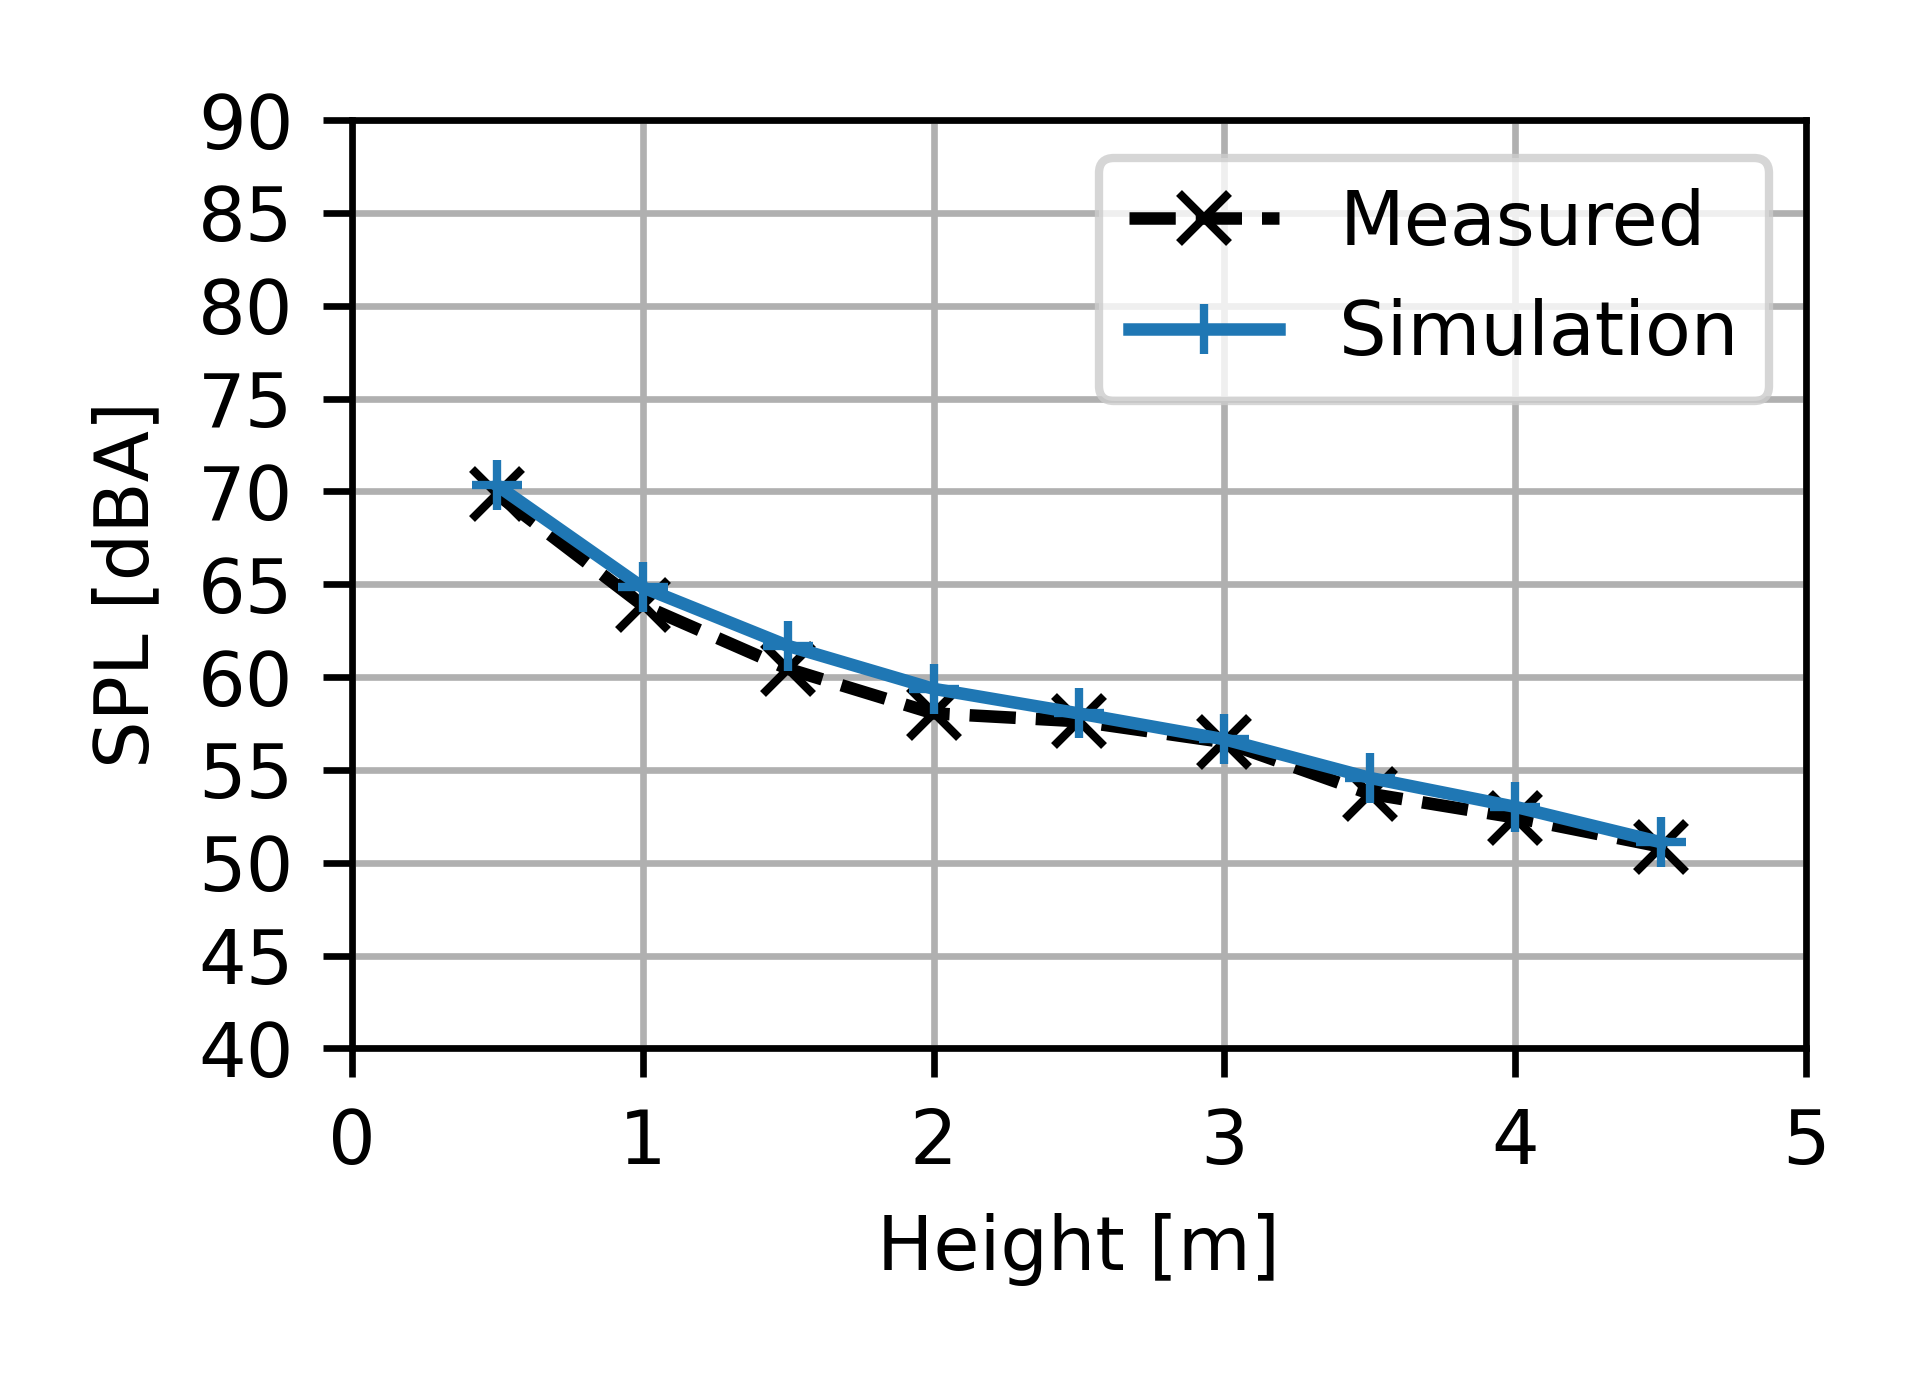
\includegraphics{fig/chap5/initial_model/third_octave_over_height/125_Hz.png}
		\caption{125 Hz}
	\end{subfigure}
	\begin{subfigure}[b]{0.49\textwidth}
		\centering
		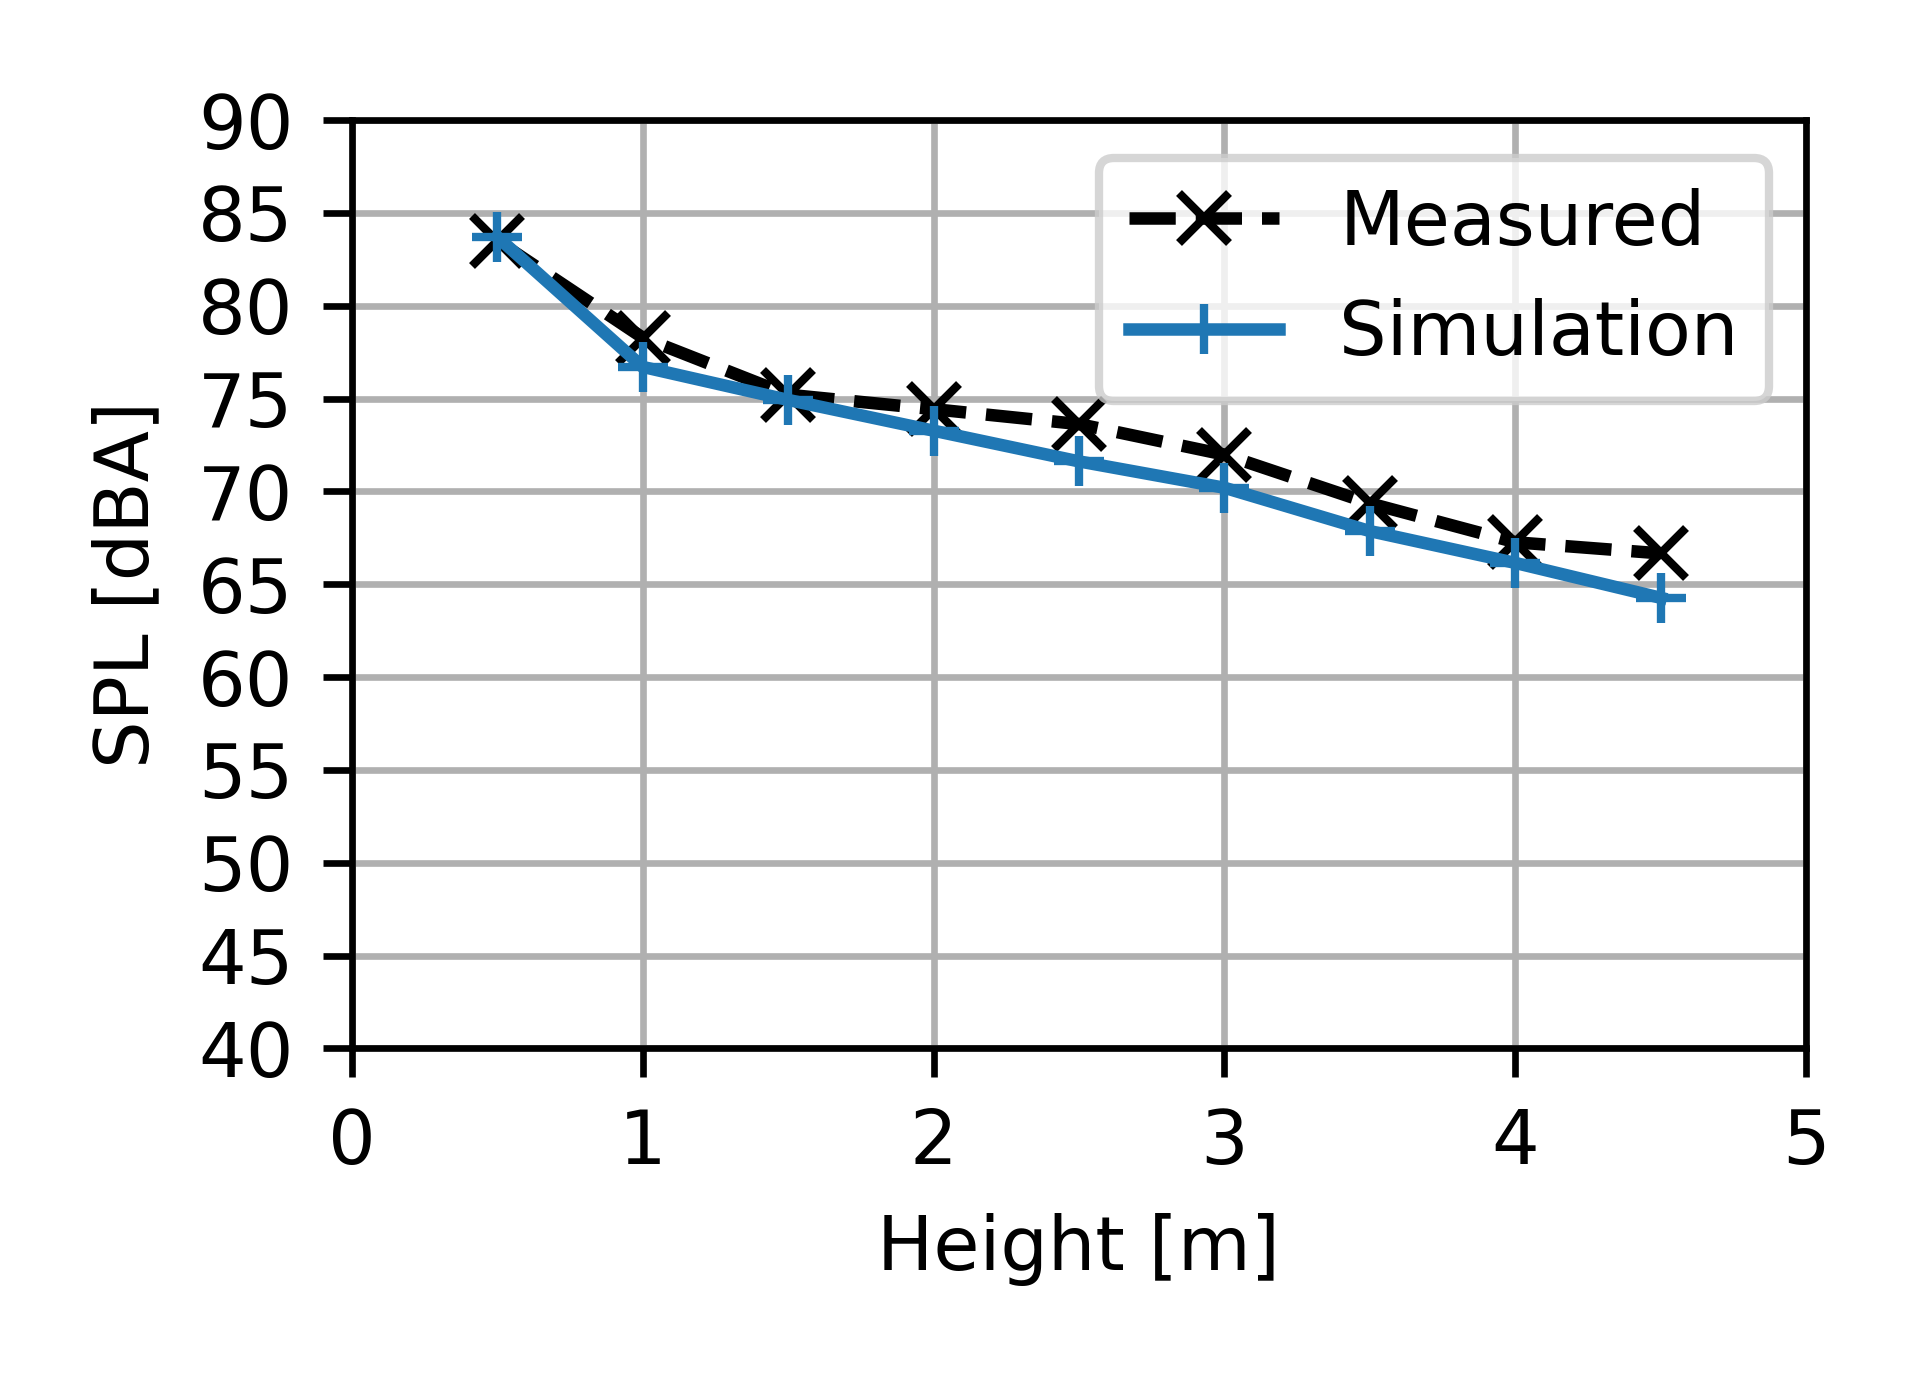
\includegraphics{fig/chap5/initial_model/third_octave_over_height/400_Hz.png}
		\caption{400 Hz}
	\end{subfigure}
	\begin{subfigure}[b]{0.49\textwidth}
		\centering
		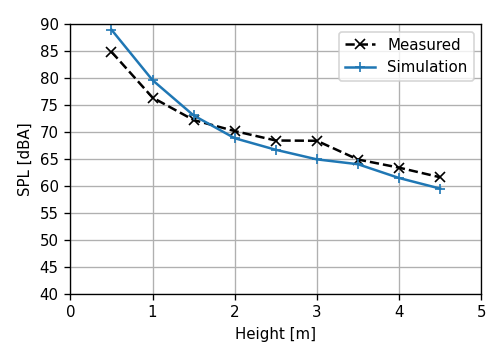
\includegraphics{fig/chap5/initial_model/third_octave_over_height/1250_Hz.png}
		\caption{1250 Hz}
	\end{subfigure}
	\begin{subfigure}[b]{0.49\textwidth}
		\centering
		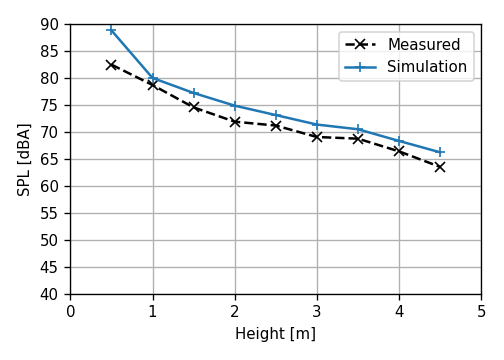
\includegraphics{fig/chap5/initial_model/third_octave_over_height/2000_Hz.png}
		\caption{2000 Hz}
	\end{subfigure}
	\caption{Sound distribution at measurement position a, comparison between predictions obtained from the initial finite element model with the measurements. A-weighted SPL in one-third octave bands, dBA ref 20 $\mu$Pa.}
	\label{fig:third_octave_over_height}
\end{figure}


\begin{figure}[H]
	\centering
	\begin{subfigure}[b]{0.49\textwidth}
		\centering
		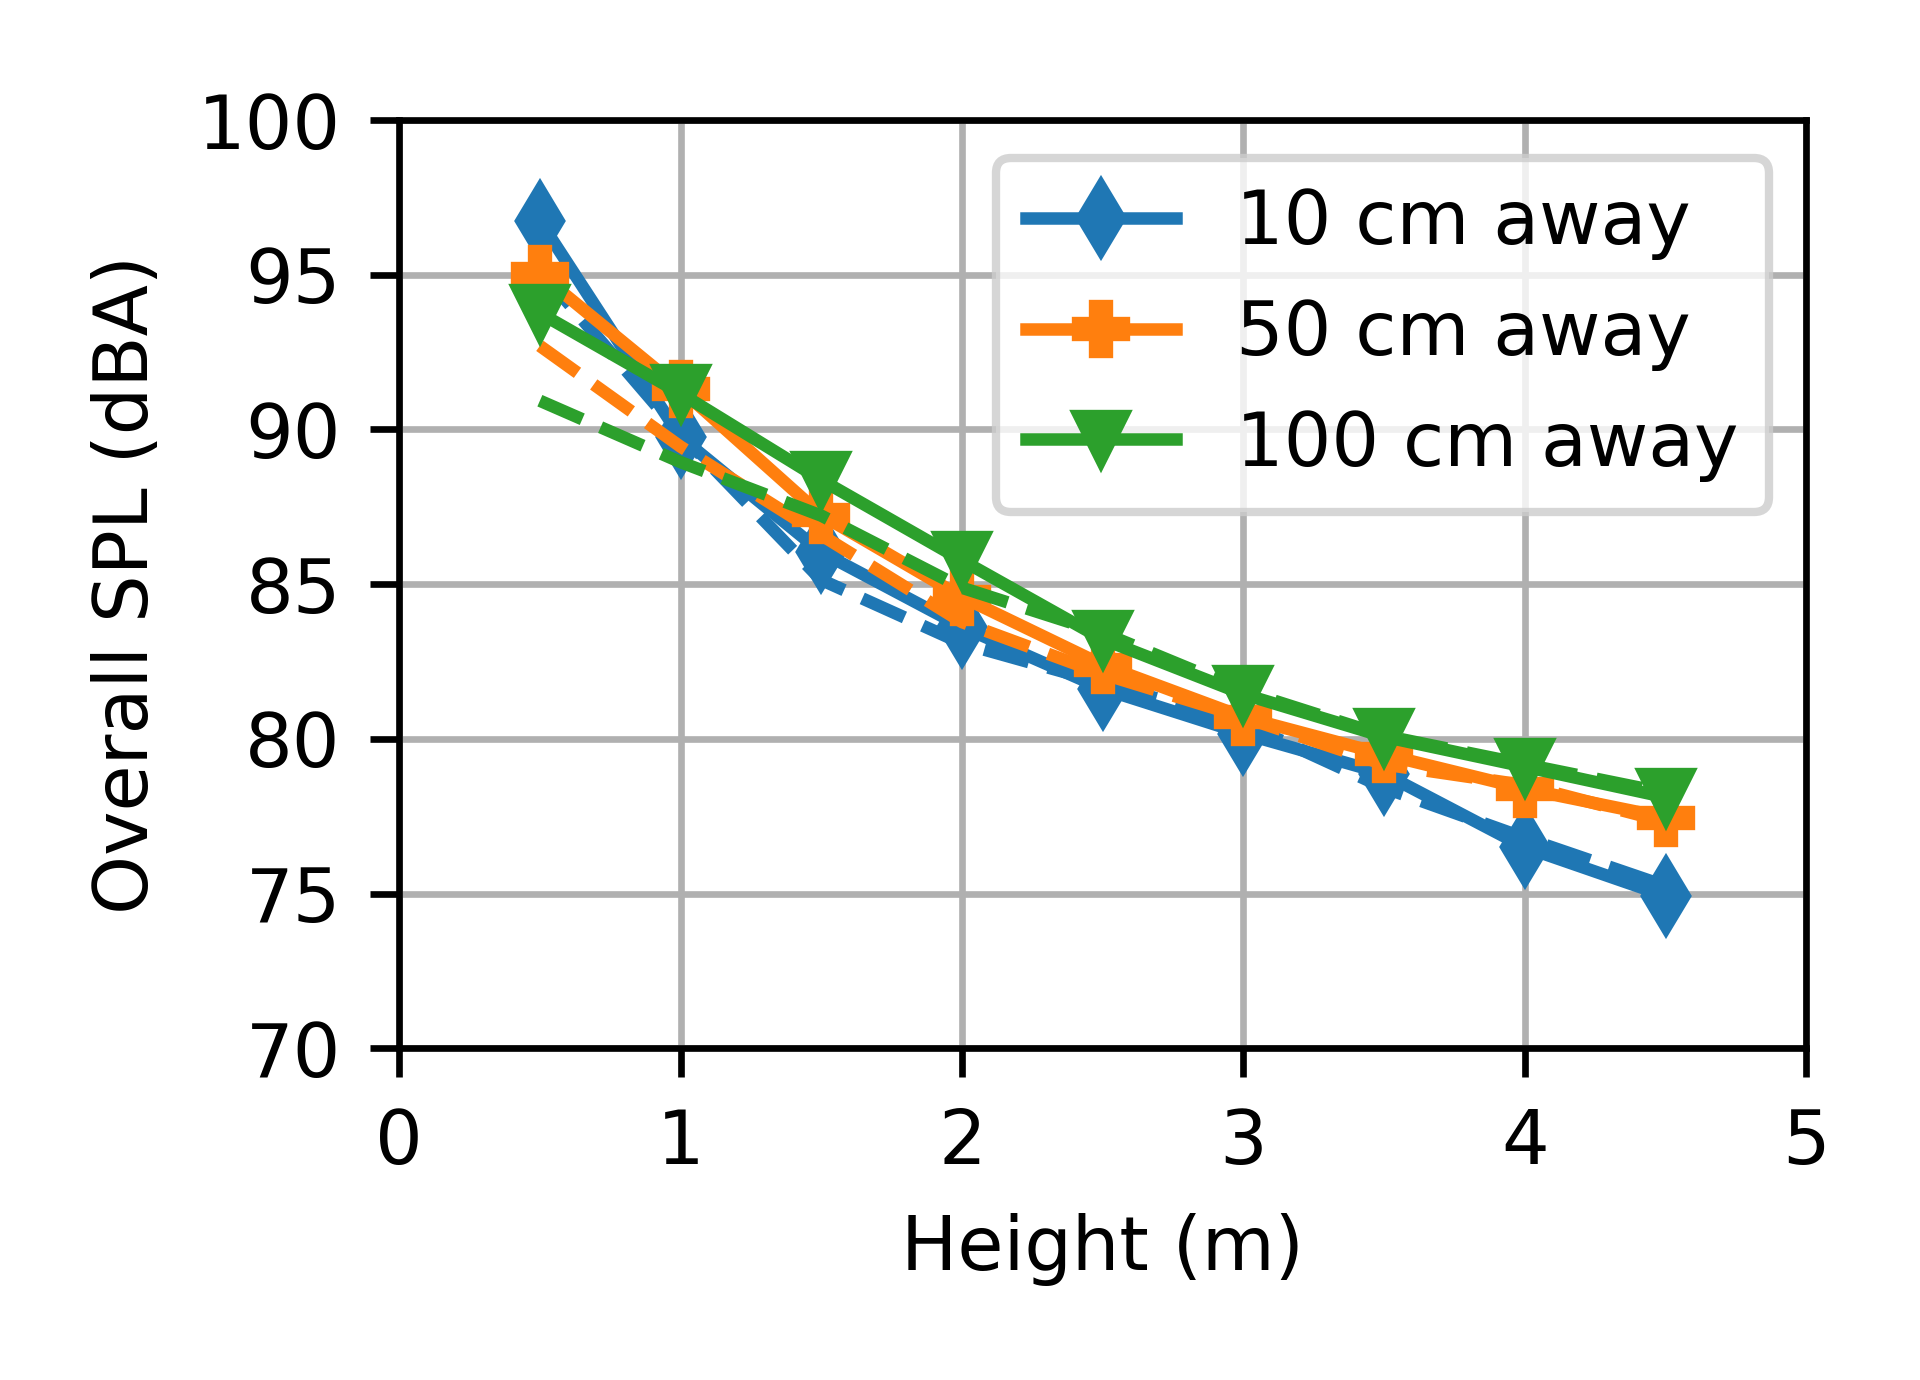
\includegraphics{fig/chap5/initial_model/overall_SPL/all_pos.png}
		%\caption{2000 Hz}
	\end{subfigure}
	\begin{subfigure}[b]{0.49\textwidth}
		\centering
		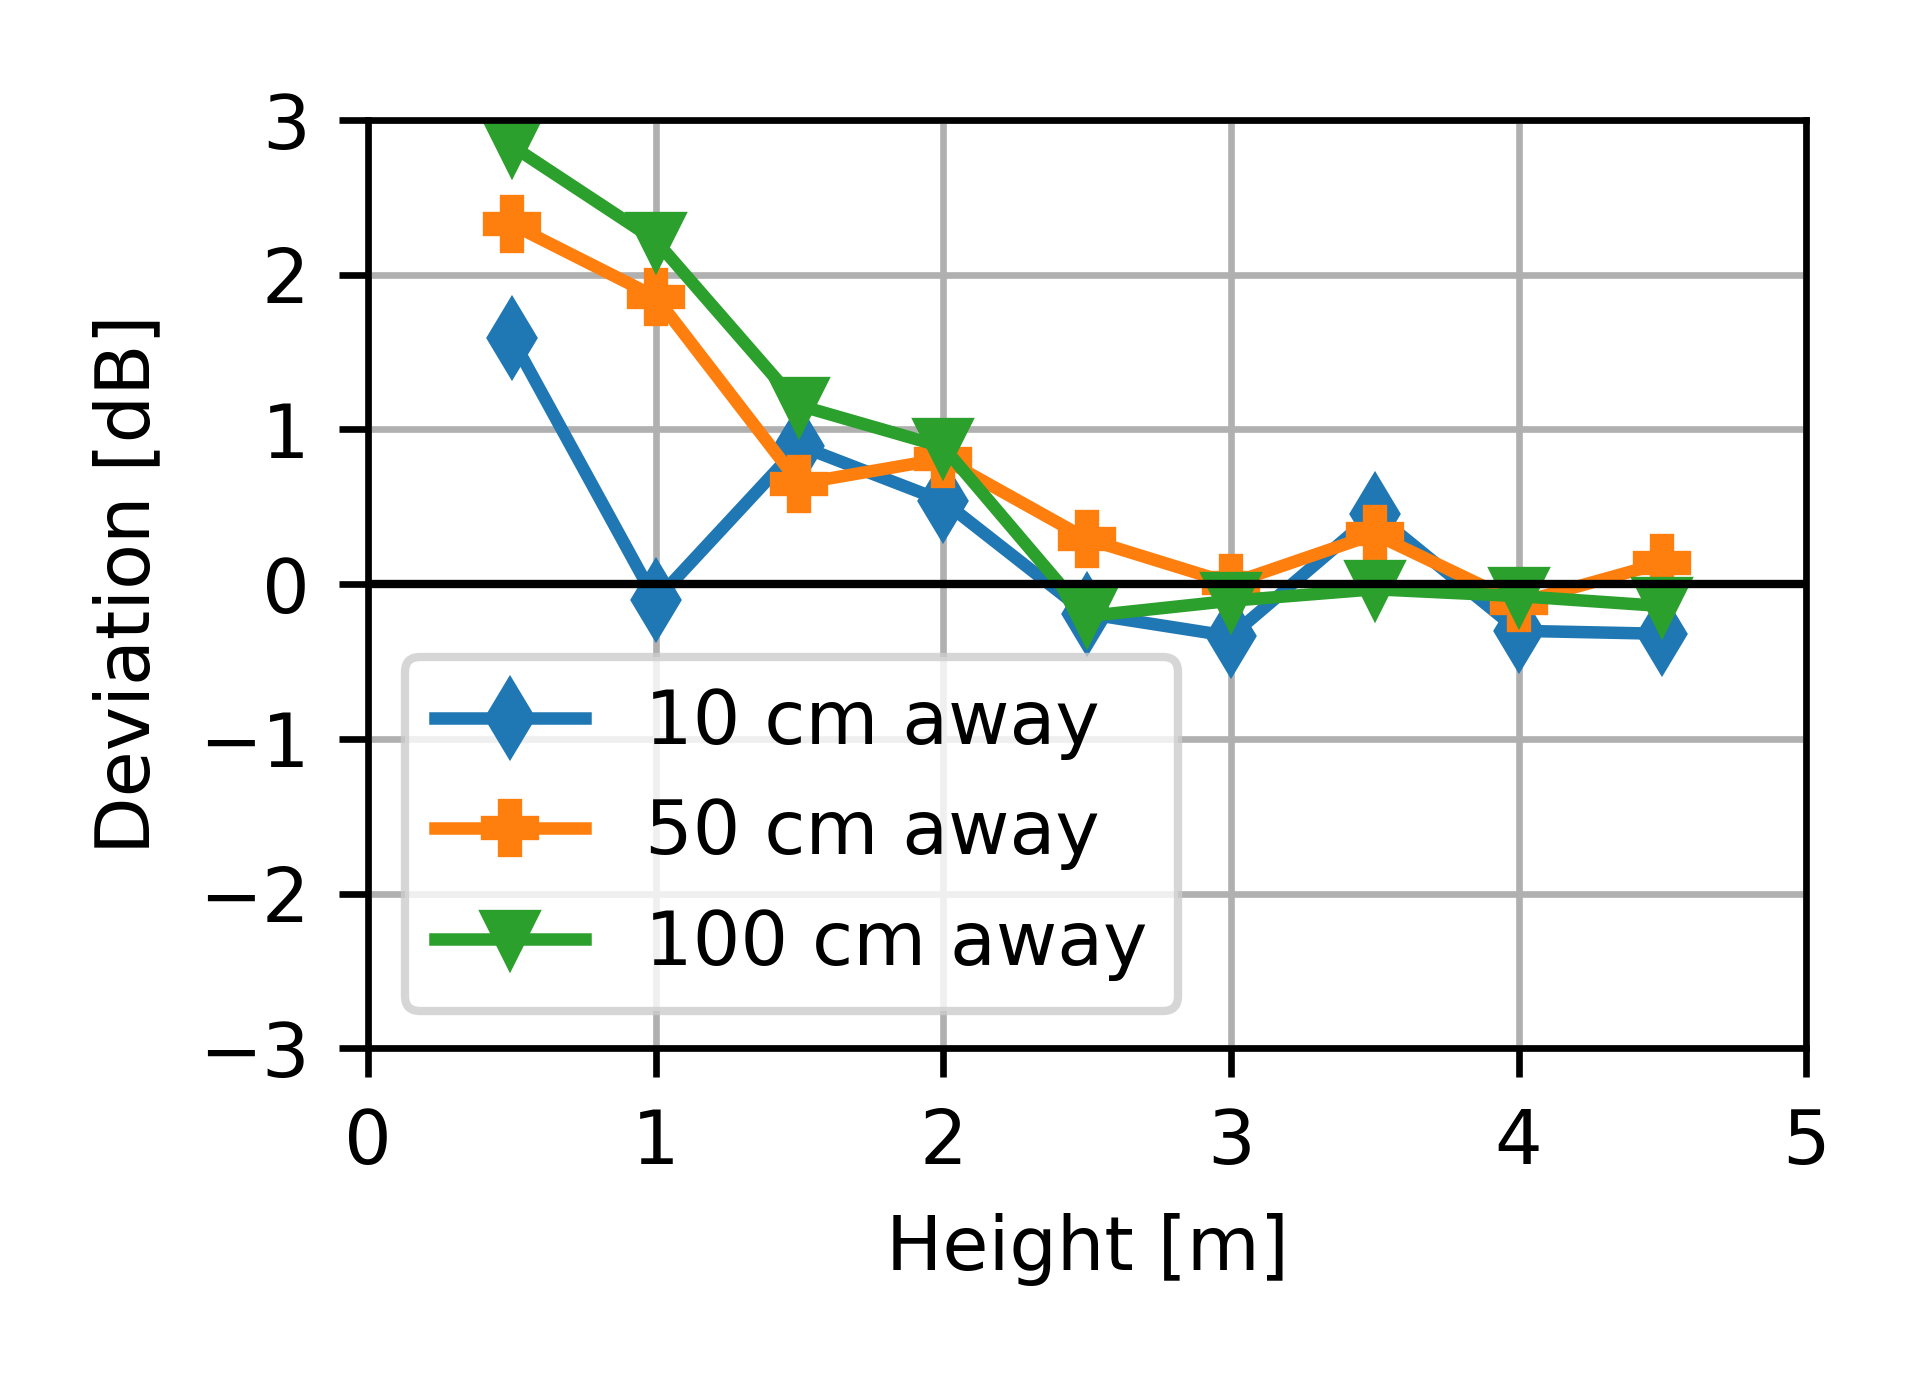
\includegraphics{fig/chap5/initial_model/overall_SPL/deviation.png}
		%\caption{2000 Hz}
	\end{subfigure}
	\caption{Comparison of overall SPL in dBA ref 20 $\mu$Pa. Left: overall SPL as a function of height at various measurement positions (dashed curves: measurement; solid curves: simulation) Right: deviation between simulation and measurement results}
	\label{fig:overall_SPL}
\end{figure}

\begin{figure}[H]
	\centering
	\begin{subfigure}[b]{0.49\textwidth}
		\centering
		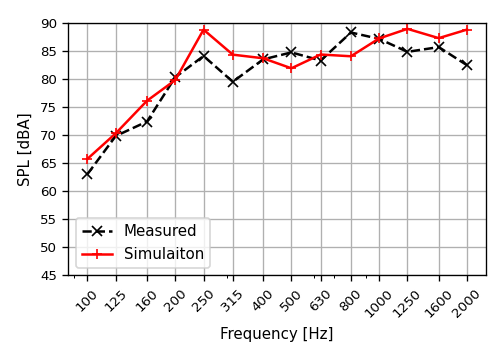
\includegraphics{fig/chap5/initial_model/freq_spectrum/pos_10cm_0pt5m.png}
		\caption{0.5 m}
	\end{subfigure}
	\begin{subfigure}[b]{0.49\textwidth}
		\centering
		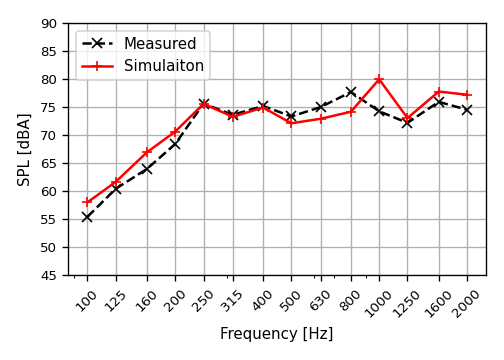
\includegraphics{fig/chap5/initial_model/freq_spectrum/pos_10cm_1pt5m.png}
		\caption{1.5 m}
	\end{subfigure}
	\begin{subfigure}[b]{0.49\textwidth}
		\centering
		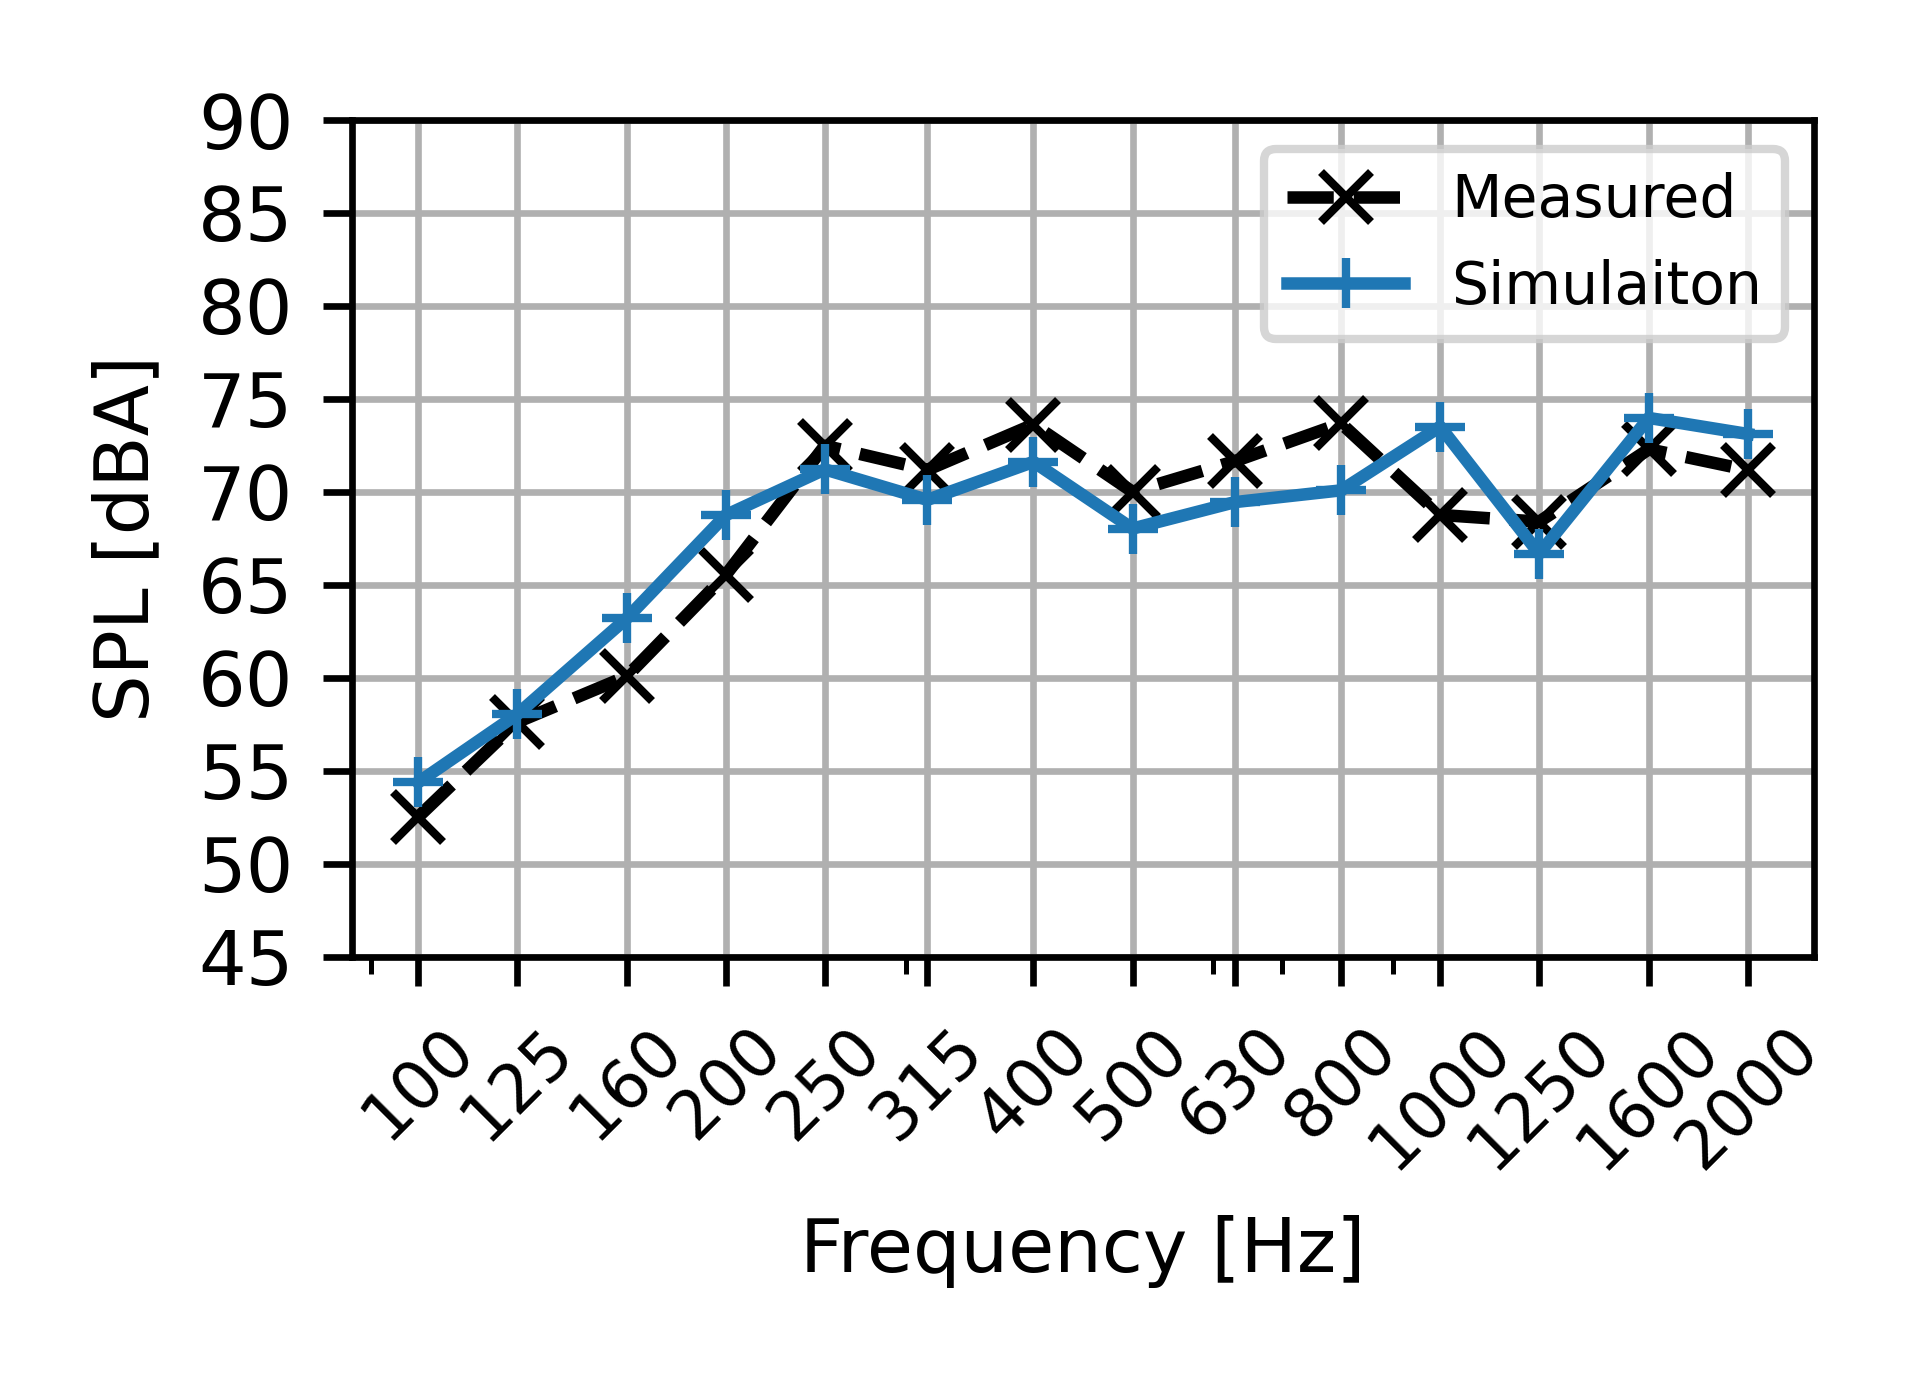
\includegraphics{fig/chap5/initial_model/freq_spectrum/pos_10cm_2pt5m.png}
		\caption{2.5 m}
	\end{subfigure}
	\begin{subfigure}[b]{0.49\textwidth}
		\centering
		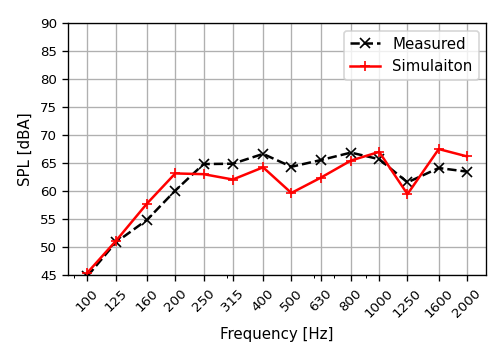
\includegraphics{fig/chap5/initial_model/freq_spectrum/pos_10cm_4pt5m.png}
		\caption{4.5 m}
	\end{subfigure}
	\caption{Comparison of overall SPL in dBA ref 20 $\mu$Pa. Left: overall SPL as a function of height at various measurement positions (dashed curves: measurement; solid curves: simulation) Right: deviation between simulation and measurement results}
	\label{fig:freq_spectrum}
\end{figure}



\begin{figure}[H]
	\centering
	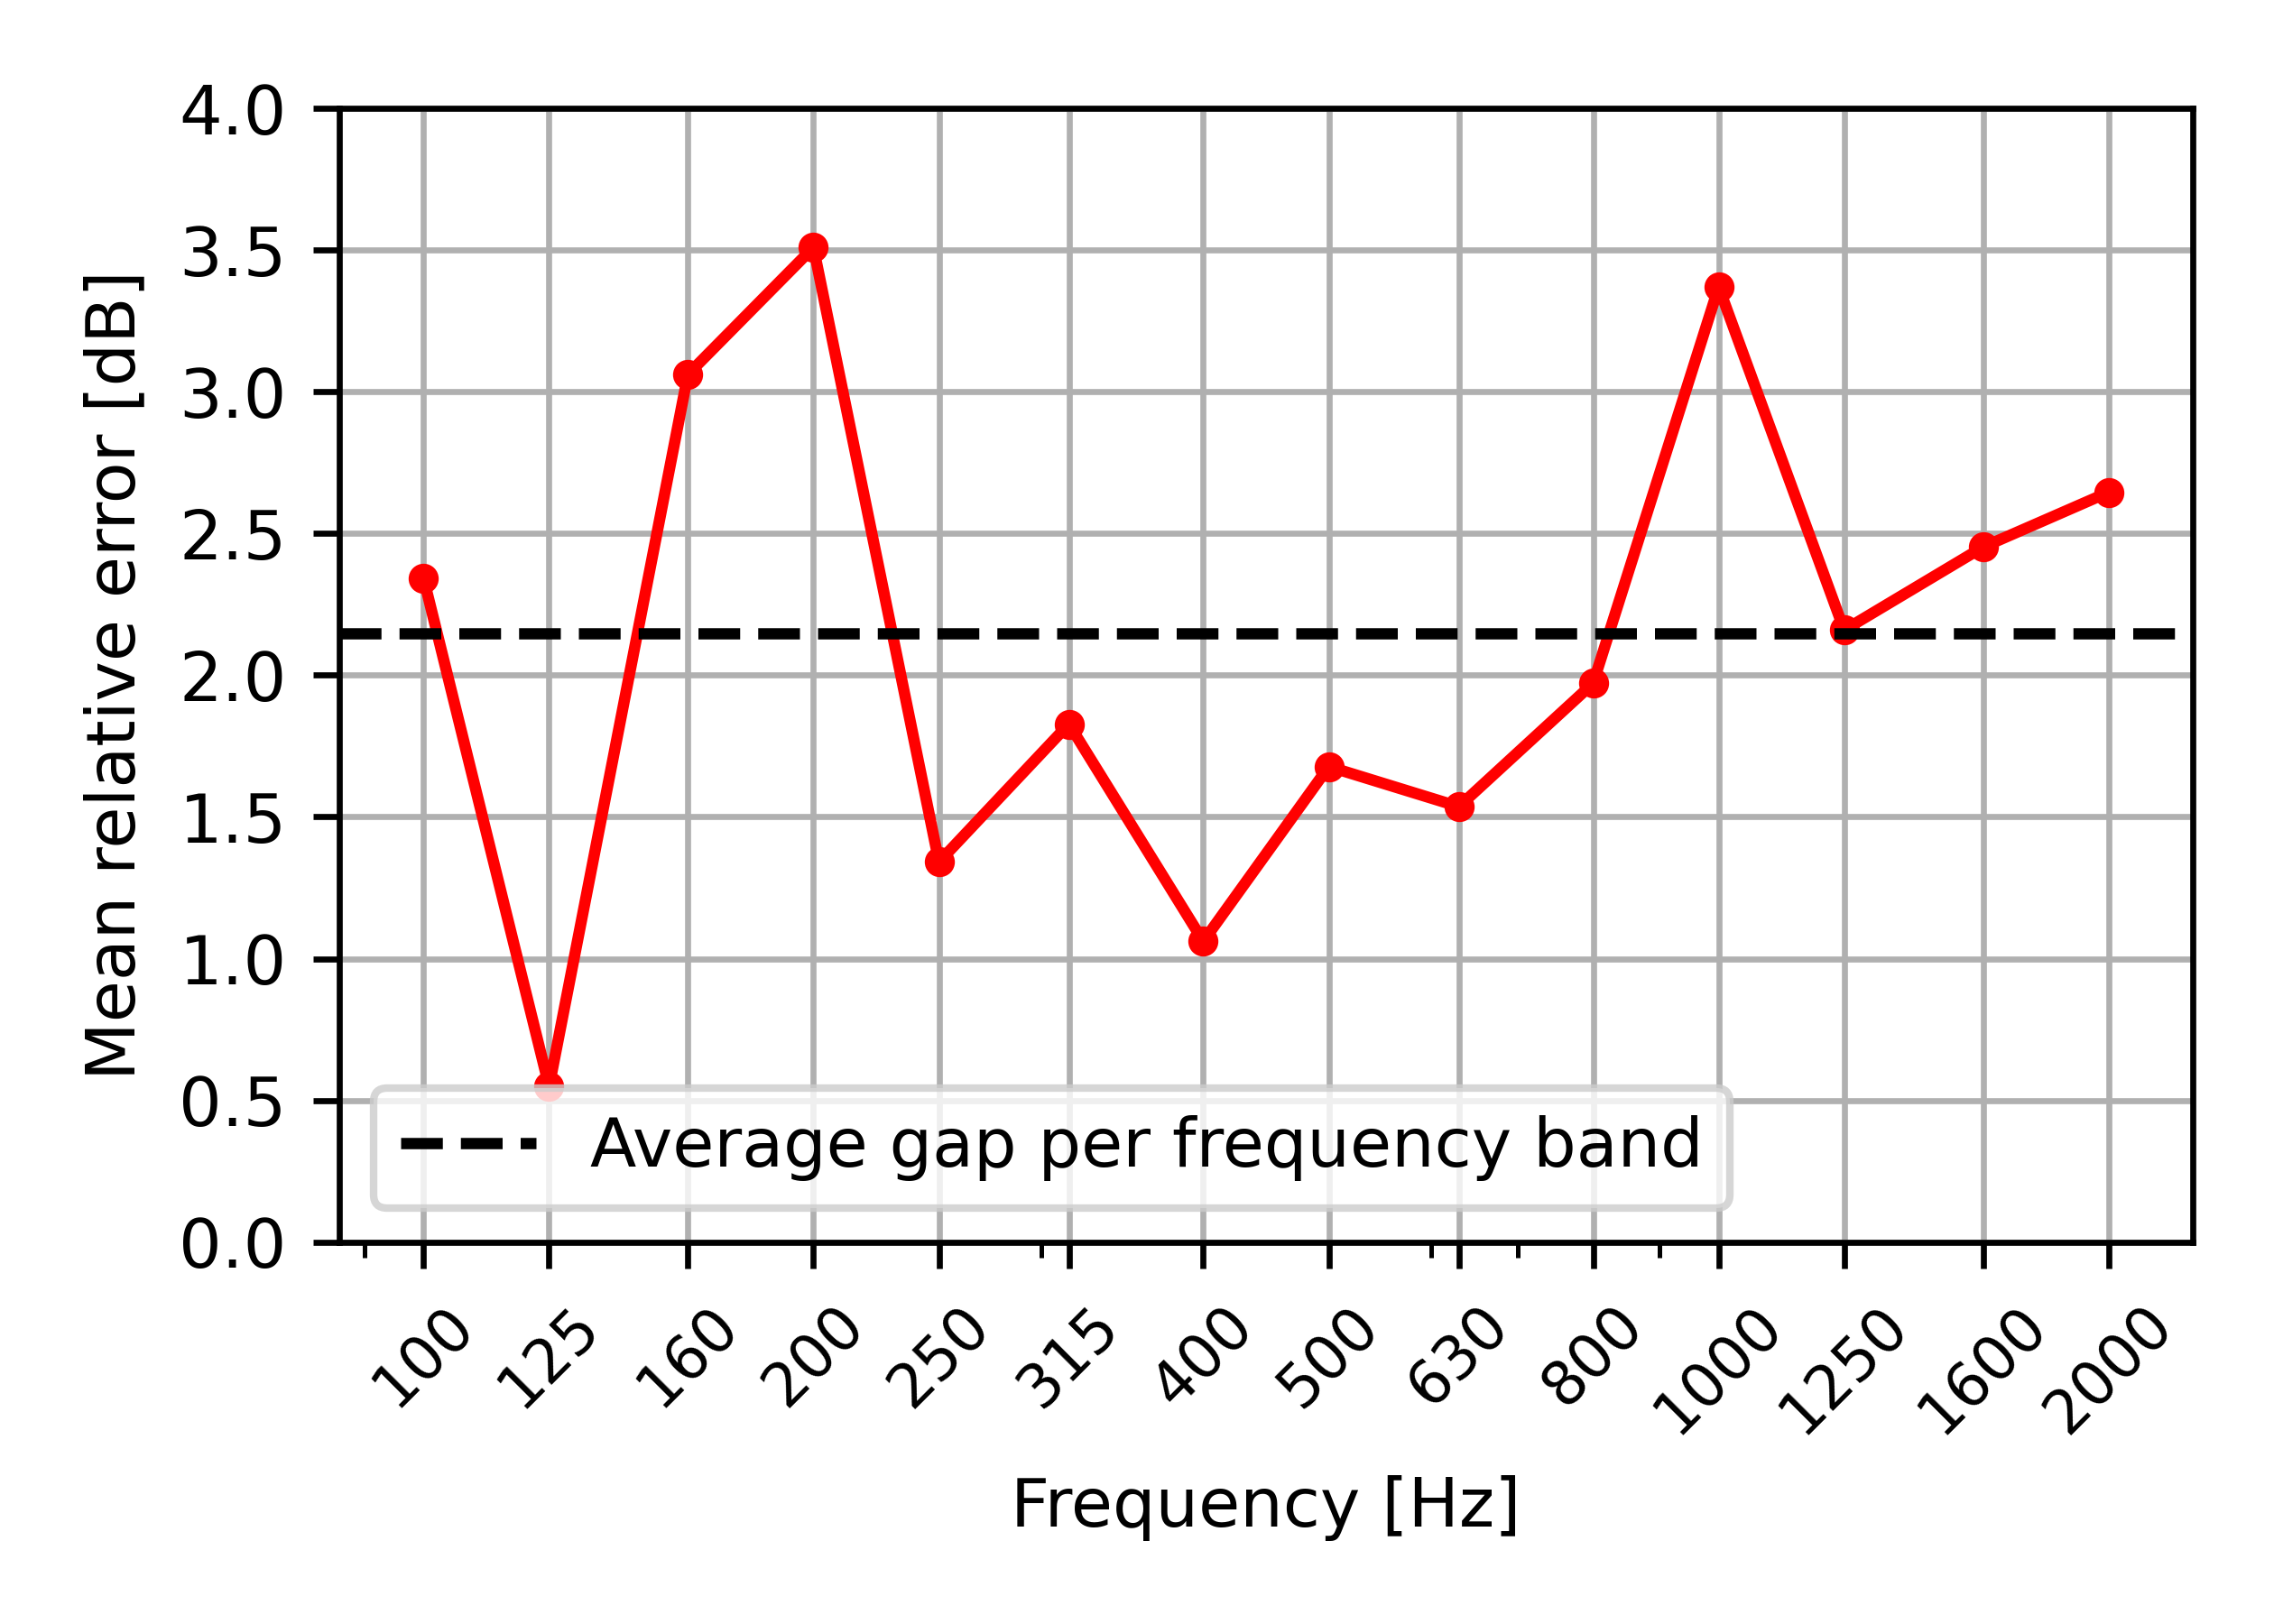
\includegraphics{fig/chap5/initial_model/freq_spectrum/average_gap.png}
	\caption{Mean relative error of 1/3-octave frequency}
	\label{fig:gap_freq_spectrum}
\end{figure}

The sound pressure level is first converted to linear scaling:

\begin{equation}
	p(\text{Pa}) = p_0 \cdot 10^{\frac{\text{SPL}}{20}} = 2\cdot10^{-5}\,\text{Pa} \cdot 10^{\frac{\text{SPL}}{20}}
\end{equation}

Mean relative error:

\begin{equation}
	\text{MRE}(p_{\text{measured}}, p_{\text{simulation}}) = \frac{1}{N} \sum_{i=0}^{N - 1} \frac{|p_{\text{simulation,}i} - p_{\text{measured,}i}|}{|p_{\text{measured,}i}|}
\end{equation}

The mean relative error  can be converted to decibel:

\begin{equation}
	\text{MRE(dB)} = 20\cdot\log_{10}(1 + \text{MRE})
\end{equation}

\begin{table}[H]
	\caption{Mean relative error of 1/3-octave frequency spectrum over all microphone positions}
	\begin{tabular}{c|cccccccccccccc}
		Freq (Hz)           & 100  & 125  & 160  & 200  & 250  & 315  & 400  & 500  & 630  & 800  & 1000 & 1250 & 1600 & 2000 \\ \hline
		MRE (dB) & 2.34 & 0.55 & 3.06 & 3.51 & 1.34 & 1.82 & 1.06 & 1.67 & 1.53 & 1.97 & 3.36 & 2.15 & 2.45 & 2.65
	\end{tabular}
\end{table}

\begin{table}[H]
	\centering
	\caption{Average gap per frequency band and mean relative error of overall SPL of initial model}
	\begin{tabular}{c|c}
		Average gap per  frequency band (dB) & Mean relative error of overall SPL (dB) \\ \hline
		$2.14\pm1$                               & $0.73\pm0.86$                             
	\end{tabular}
\end{table}


\section{Effect of geometric variation}

\begin{figure}[H]
	\centering
	\begin{subfigure}[b]{0.49\textwidth}
		\centering
		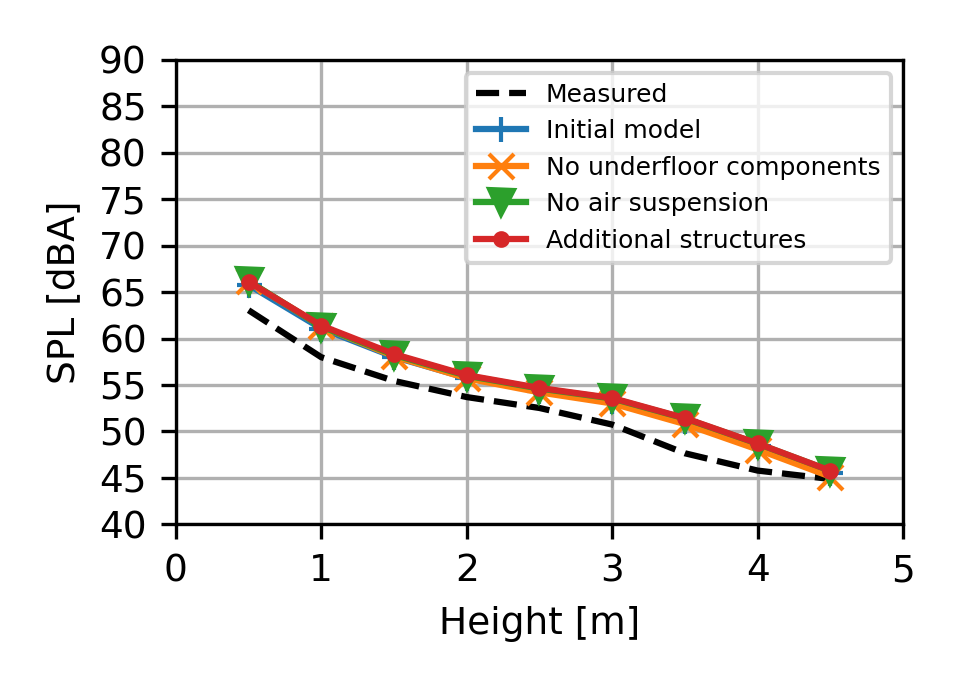
\includegraphics{fig/chap5/geometry_variation/third_octave_over_height/100_Hz.png}
		\caption{100 Hz}
	\end{subfigure}
	\begin{subfigure}[b]{0.49\textwidth}
		\centering
		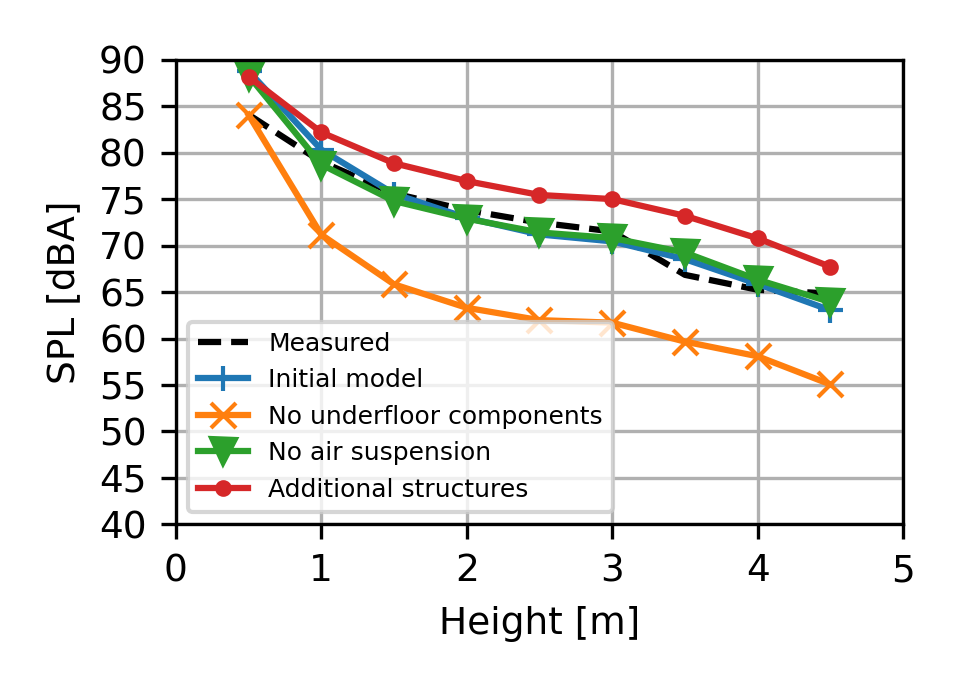
\includegraphics{fig/chap5/geometry_variation/third_octave_over_height/250_Hz.png}
		\caption{250 Hz}
	\end{subfigure}
	\begin{subfigure}[b]{0.49\textwidth}
		\centering
		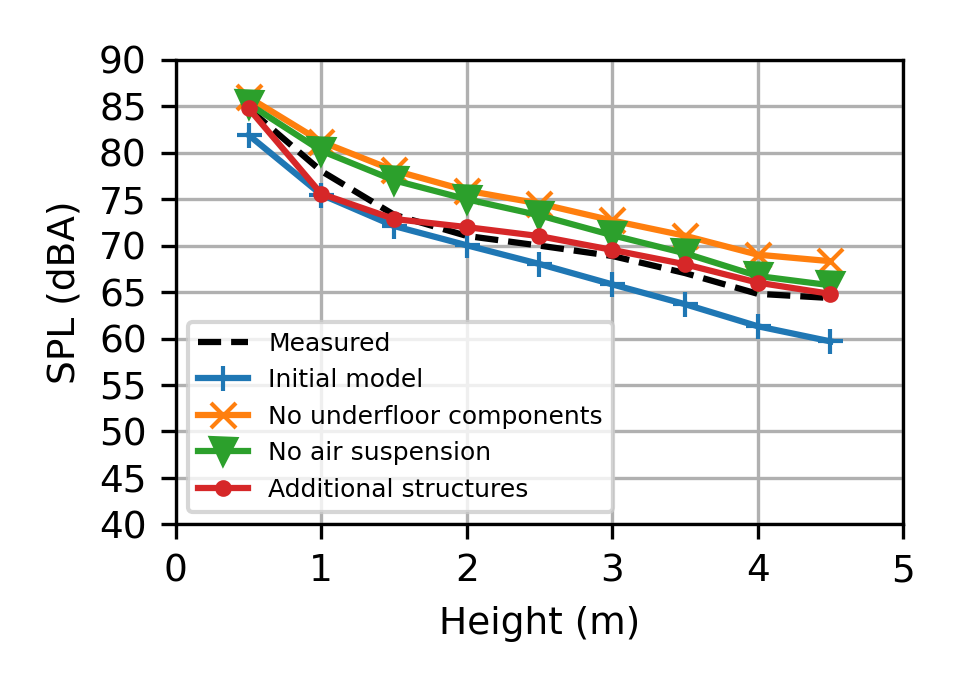
\includegraphics{fig/chap5/geometry_variation/third_octave_over_height/500_Hz.png}
		\caption{500 Hz}
	\end{subfigure}
	\begin{subfigure}[b]{0.49\textwidth}
		\centering
		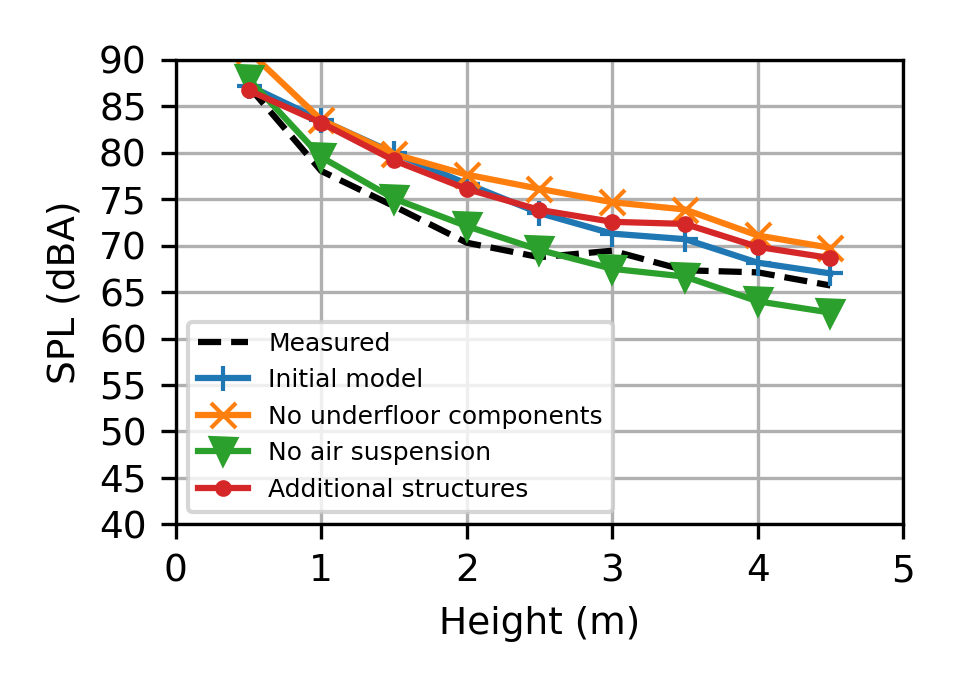
\includegraphics{fig/chap5/geometry_variation/third_octave_over_height/1000_Hz.png}
		\caption{1000 Hz}
	\end{subfigure}
	\caption{Sound distribution at measurement position a, comparison between predictions obtained from the initial finite element model with the measurements. A-weighted SPL in one-third octave bands, dBA ref 20 $\mu$Pa.}
	\label{fig:third_octave_over_height_geometry_variation}
\end{figure}

\begin{figure}[H]
	\centering
	\begin{subfigure}[b]{\textwidth}
		\centering
		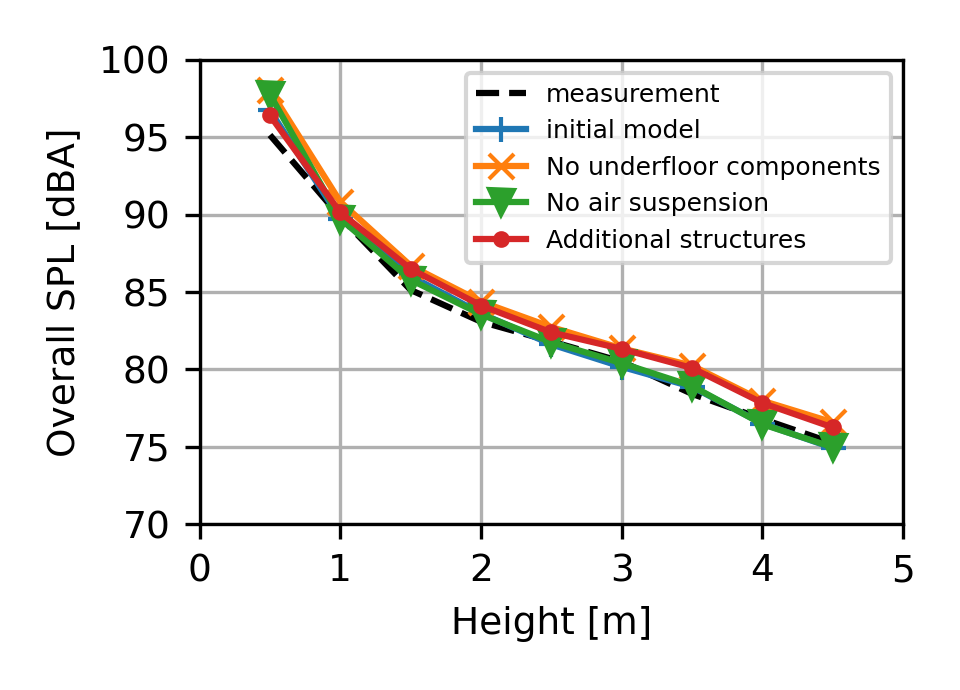
\includegraphics[width=0.49\linewidth]{fig/chap5/geometry_variation/overall_SPL/pos_a.png}
		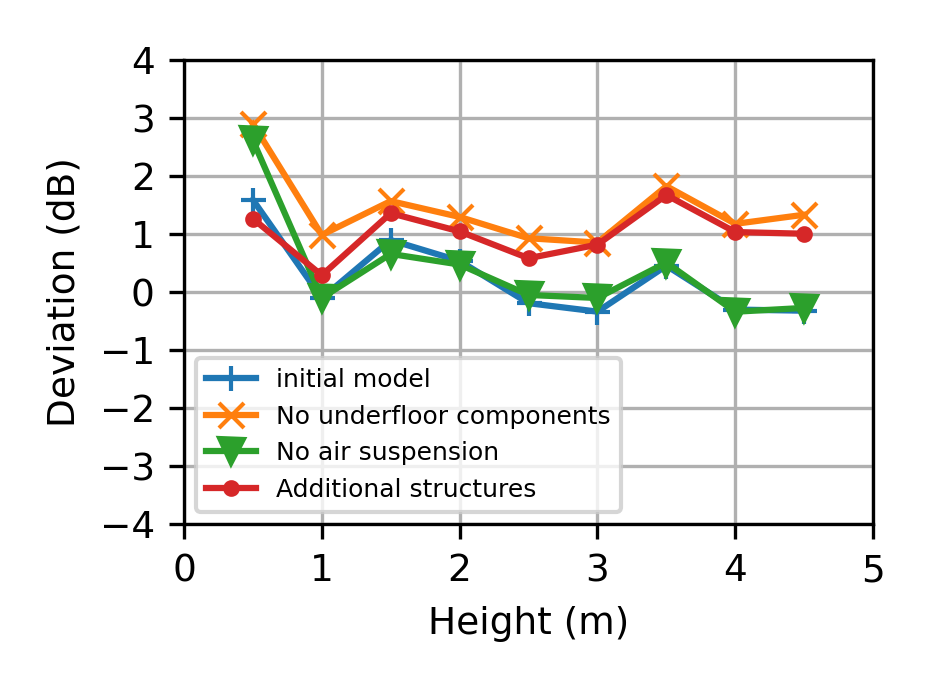
\includegraphics[width=0.49\linewidth]{fig/chap5/geometry_variation/overall_SPL/pos_a_deviation.png}
		\caption{10 cm away from carbody}
	\end{subfigure}
	\begin{subfigure}[b]{\textwidth}
		\centering
		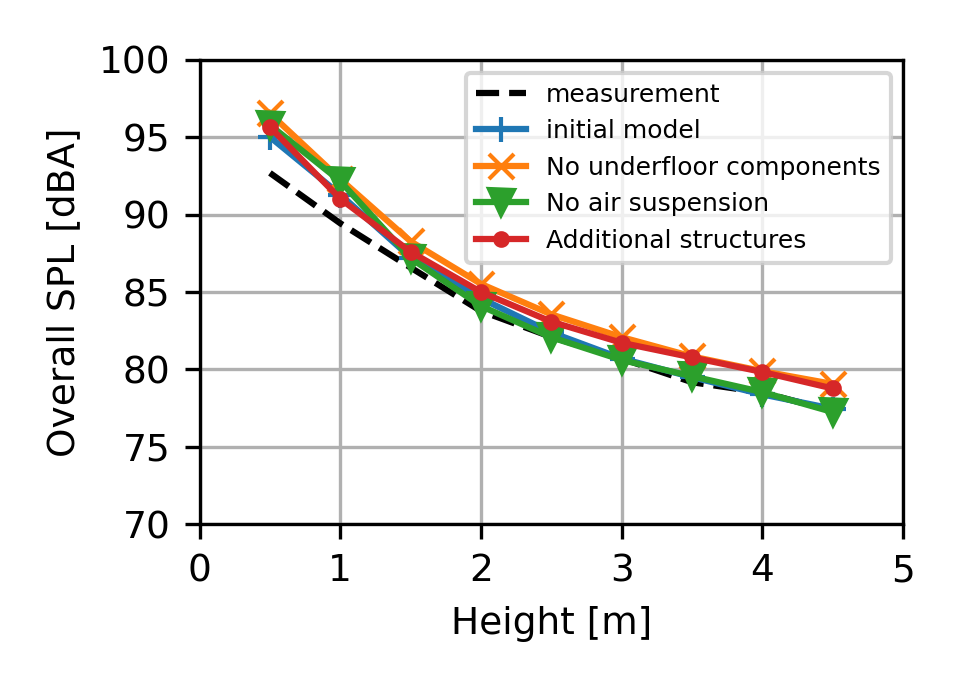
\includegraphics[width=0.49\linewidth]{fig/chap5/geometry_variation/overall_SPL/pos_f.png}
		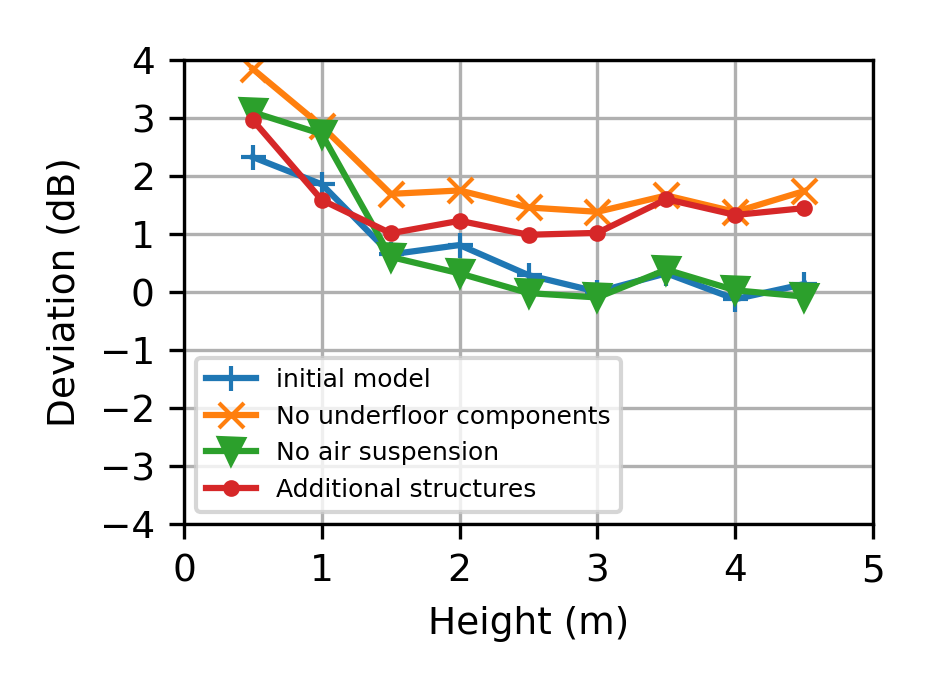
\includegraphics[width=0.49\linewidth]{fig/chap5/geometry_variation/overall_SPL/pos_f_deviation.png}
		\caption{50 cm away from carbody}
	\end{subfigure}
	\begin{subfigure}[b]{\textwidth}
		\centering
		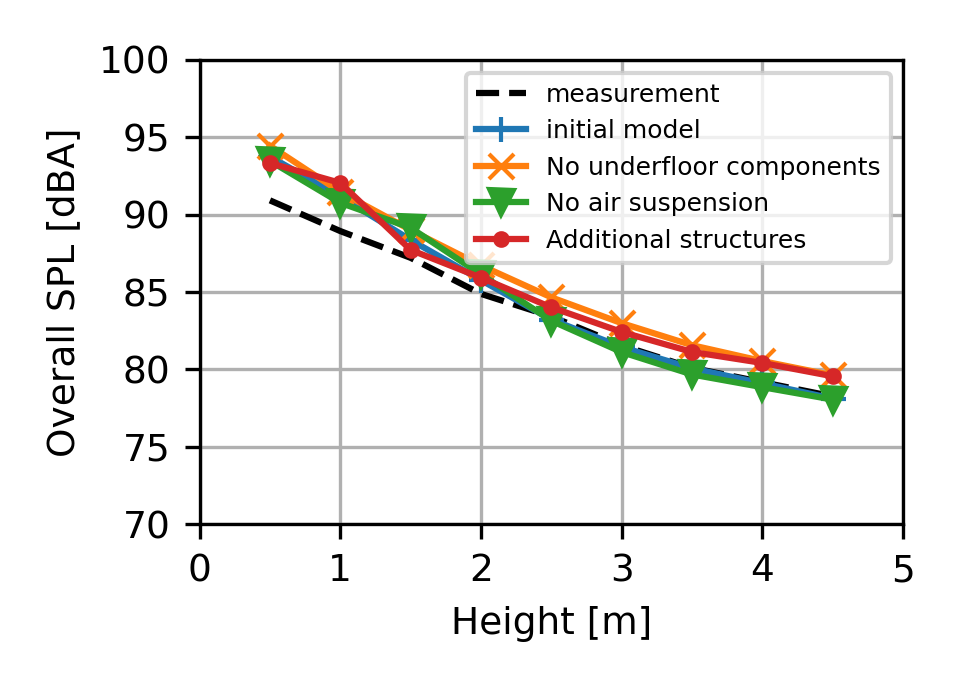
\includegraphics[width=0.49\linewidth]{fig/chap5/geometry_variation/overall_SPL/pos_g.png}
		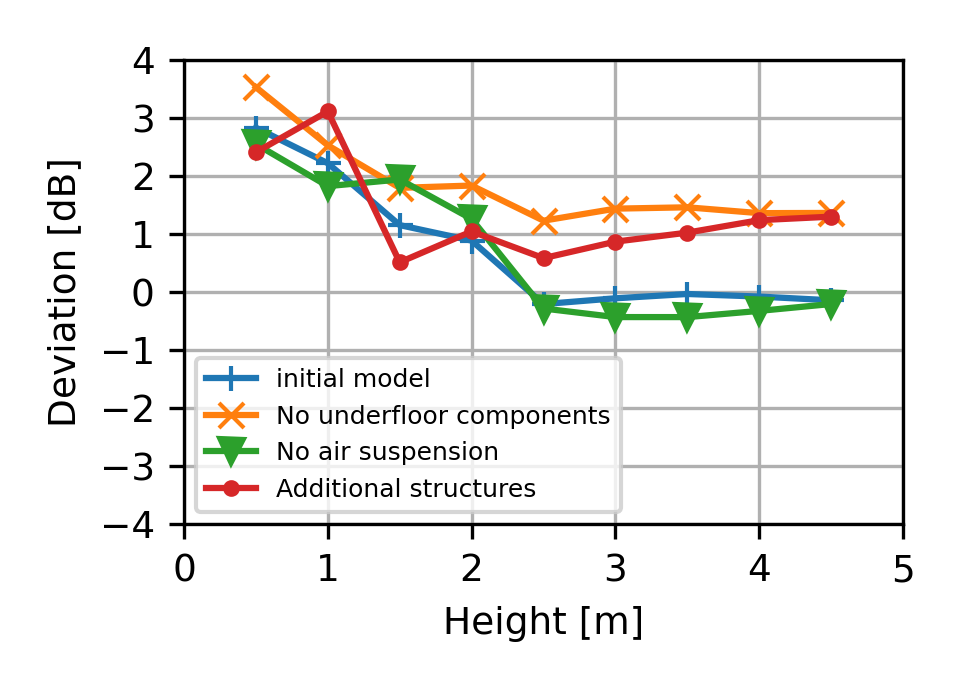
\includegraphics[width=0.49\linewidth]{fig/chap5/geometry_variation/overall_SPL/pos_g_deviation.png}
		\caption{100 cm away from carbody}
	\end{subfigure}
	\caption{Comparison of overall SPL in dBA ref 20 $\mu$Pa. Left: overall SPL as a function of height at various measurement positions (dashed curves: measurement; solid curves: simulation) Right: deviation between simulation and measurement results}
	\label{fig:overall_SPL_geometry}
\end{figure}


\begin{figure}[H]
	\centering
	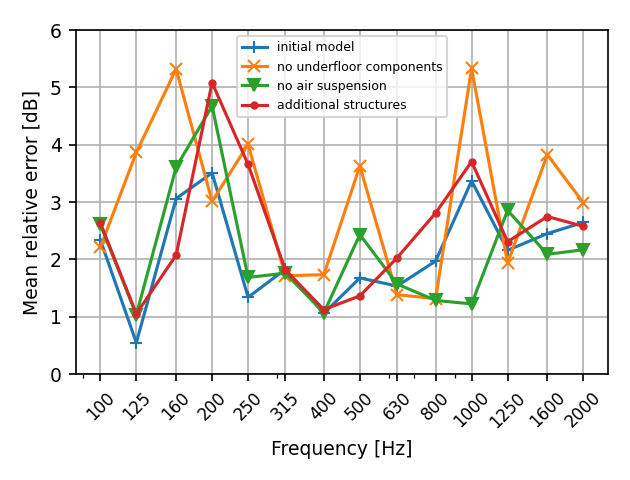
\includegraphics[width=0.7\linewidth]{fig/chap5/geometry_variation/freq_spectrum/average_gap.png}
	\caption{Mean relative error of 1/3-octave frequency}
	\label{fig:gap_freq_spectrum_geometry}
\end{figure}

\begin{table}[H]
	\centering
	\caption{Average gap per frequency band and mean relative error in overall SPL for different geometry variations}
	\begin{tabular}{c|c|c}
		Geometry name              & Average gap per frequency band (dB) & MRE overall SPL (dB) \\ \hline
		No underfloor components   & $3.12\pm1.74$                       & $1.78\pm0.91$        \\
		No air suspension          & $2.21\pm1.27$                       & $0.85\pm1.05$        \\
		Initial model              & $2.34\pm1.00$                       & $0.73\pm0.86$        \\
		With additional structures & $2.57\pm1.38$                       & $1.30\pm0.76$       
	\end{tabular}
\end{table}


\section{Effect of ground absorption}

\begin{figure}[H]
	\centering
	\begin{subfigure}[b]{\textwidth}
		\centering
		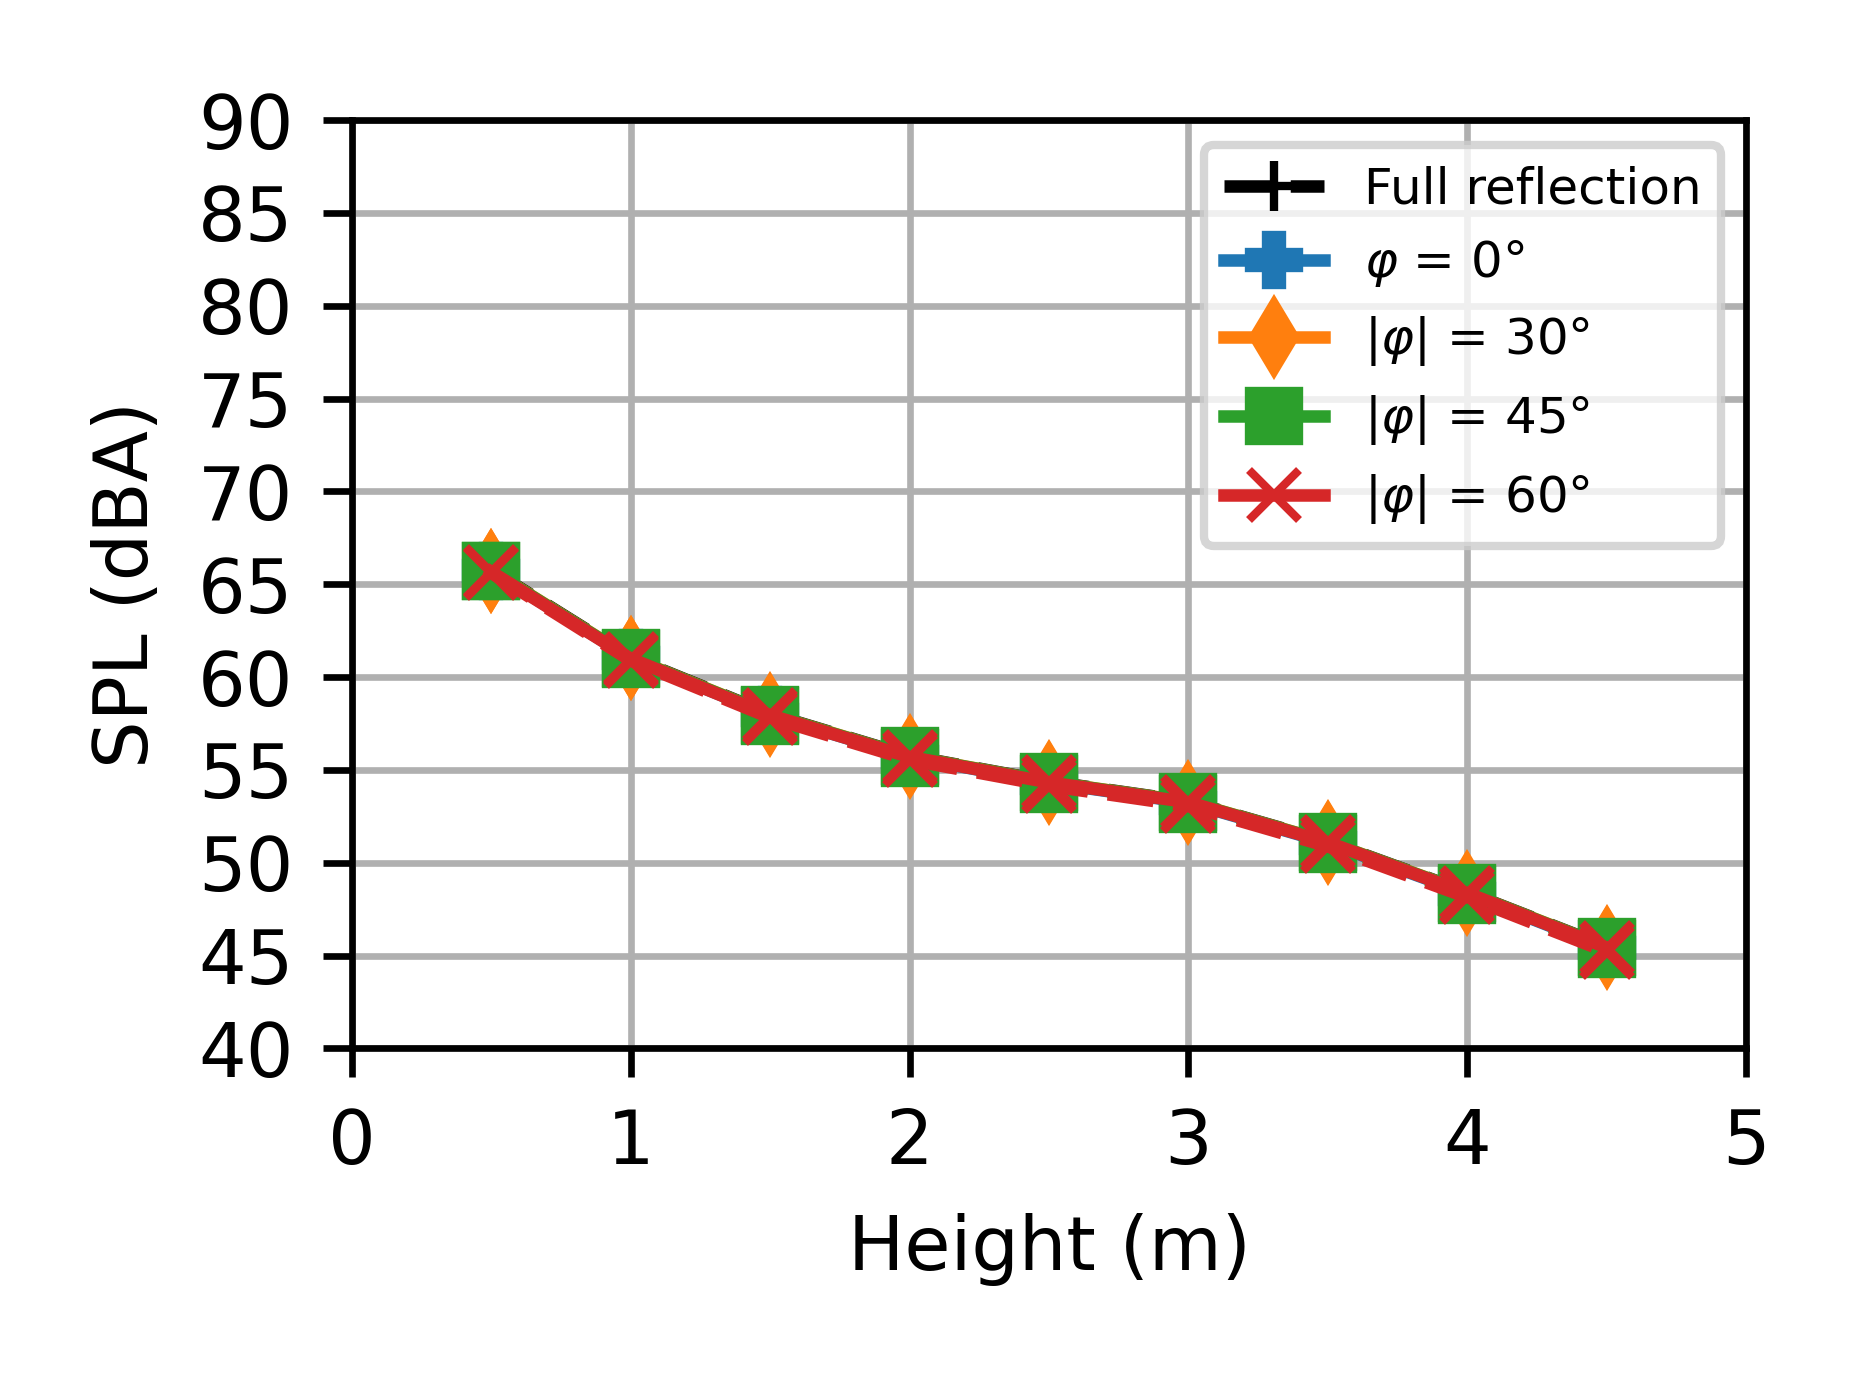
\includegraphics[width=0.49\textwidth]{fig/chap5/impedance/third_octave/SPL_100_Hz.png}
		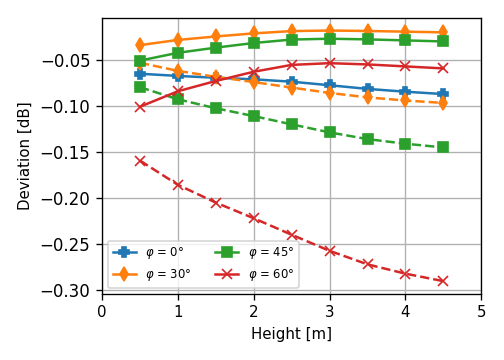
\includegraphics[width=0.49\textwidth]{fig/chap5/impedance/third_octave/deviation_100_Hz.png}
		\caption{100 Hz}
	\end{subfigure}
	\begin{subfigure}[b]{\textwidth}
		\centering
		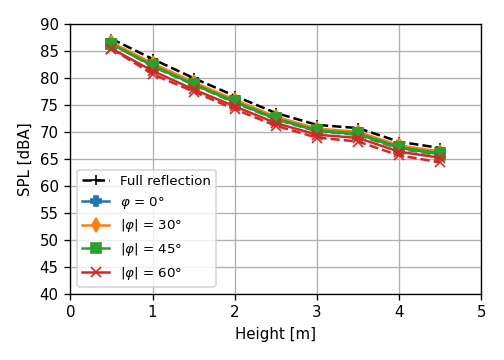
\includegraphics[width=0.49\textwidth]{fig/chap5/impedance/third_octave/SPL_1000_Hz.png}
		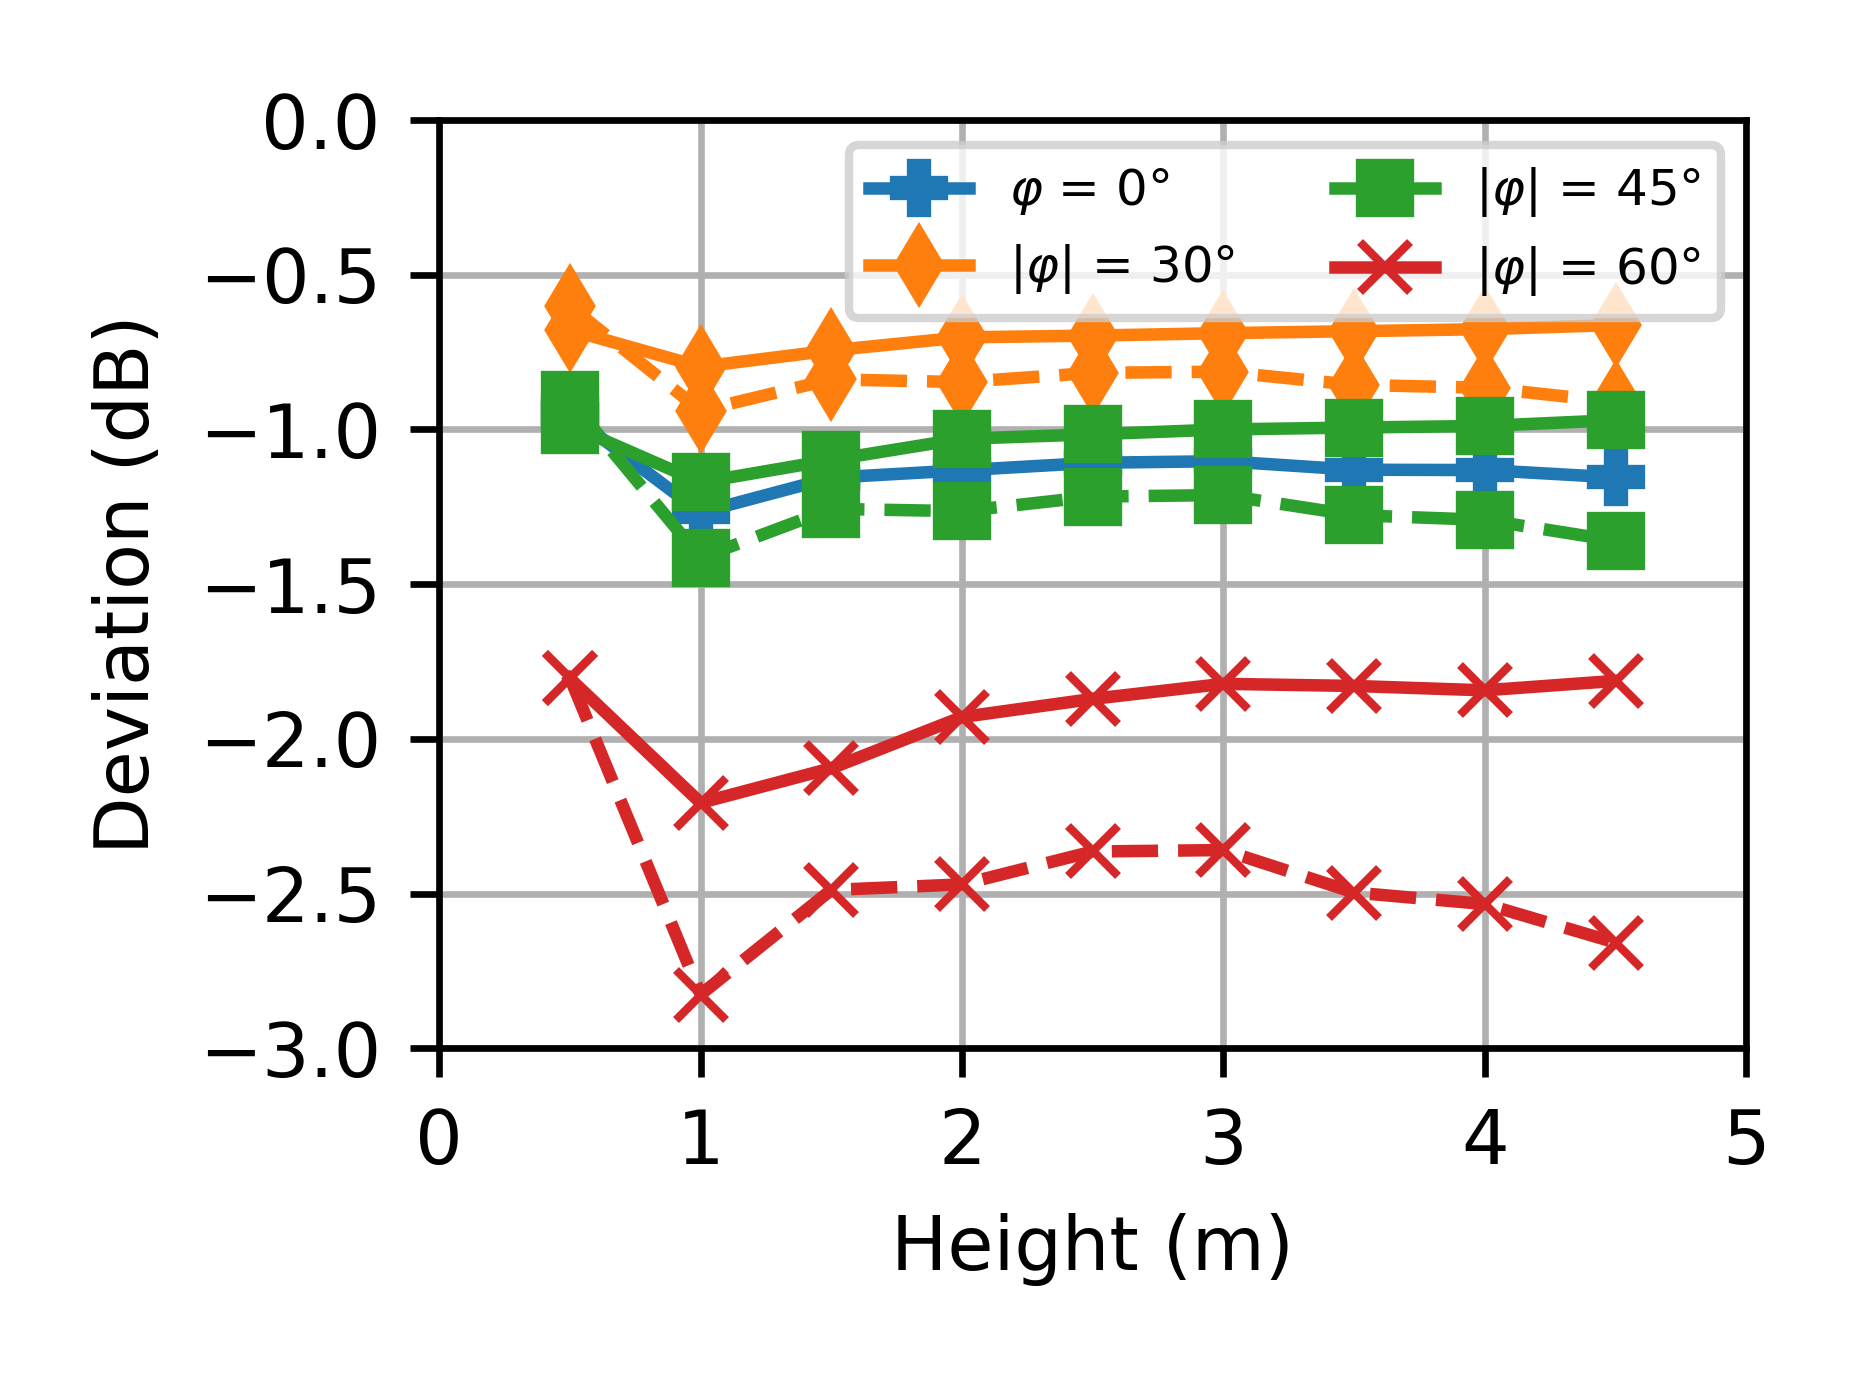
\includegraphics[width=0.49\textwidth]{fig/chap5/impedance/third_octave/deviation_1000_Hz.png}
		\caption{1000 Hz}
	\end{subfigure}
	\begin{subfigure}[b]{\textwidth}
		\centering
		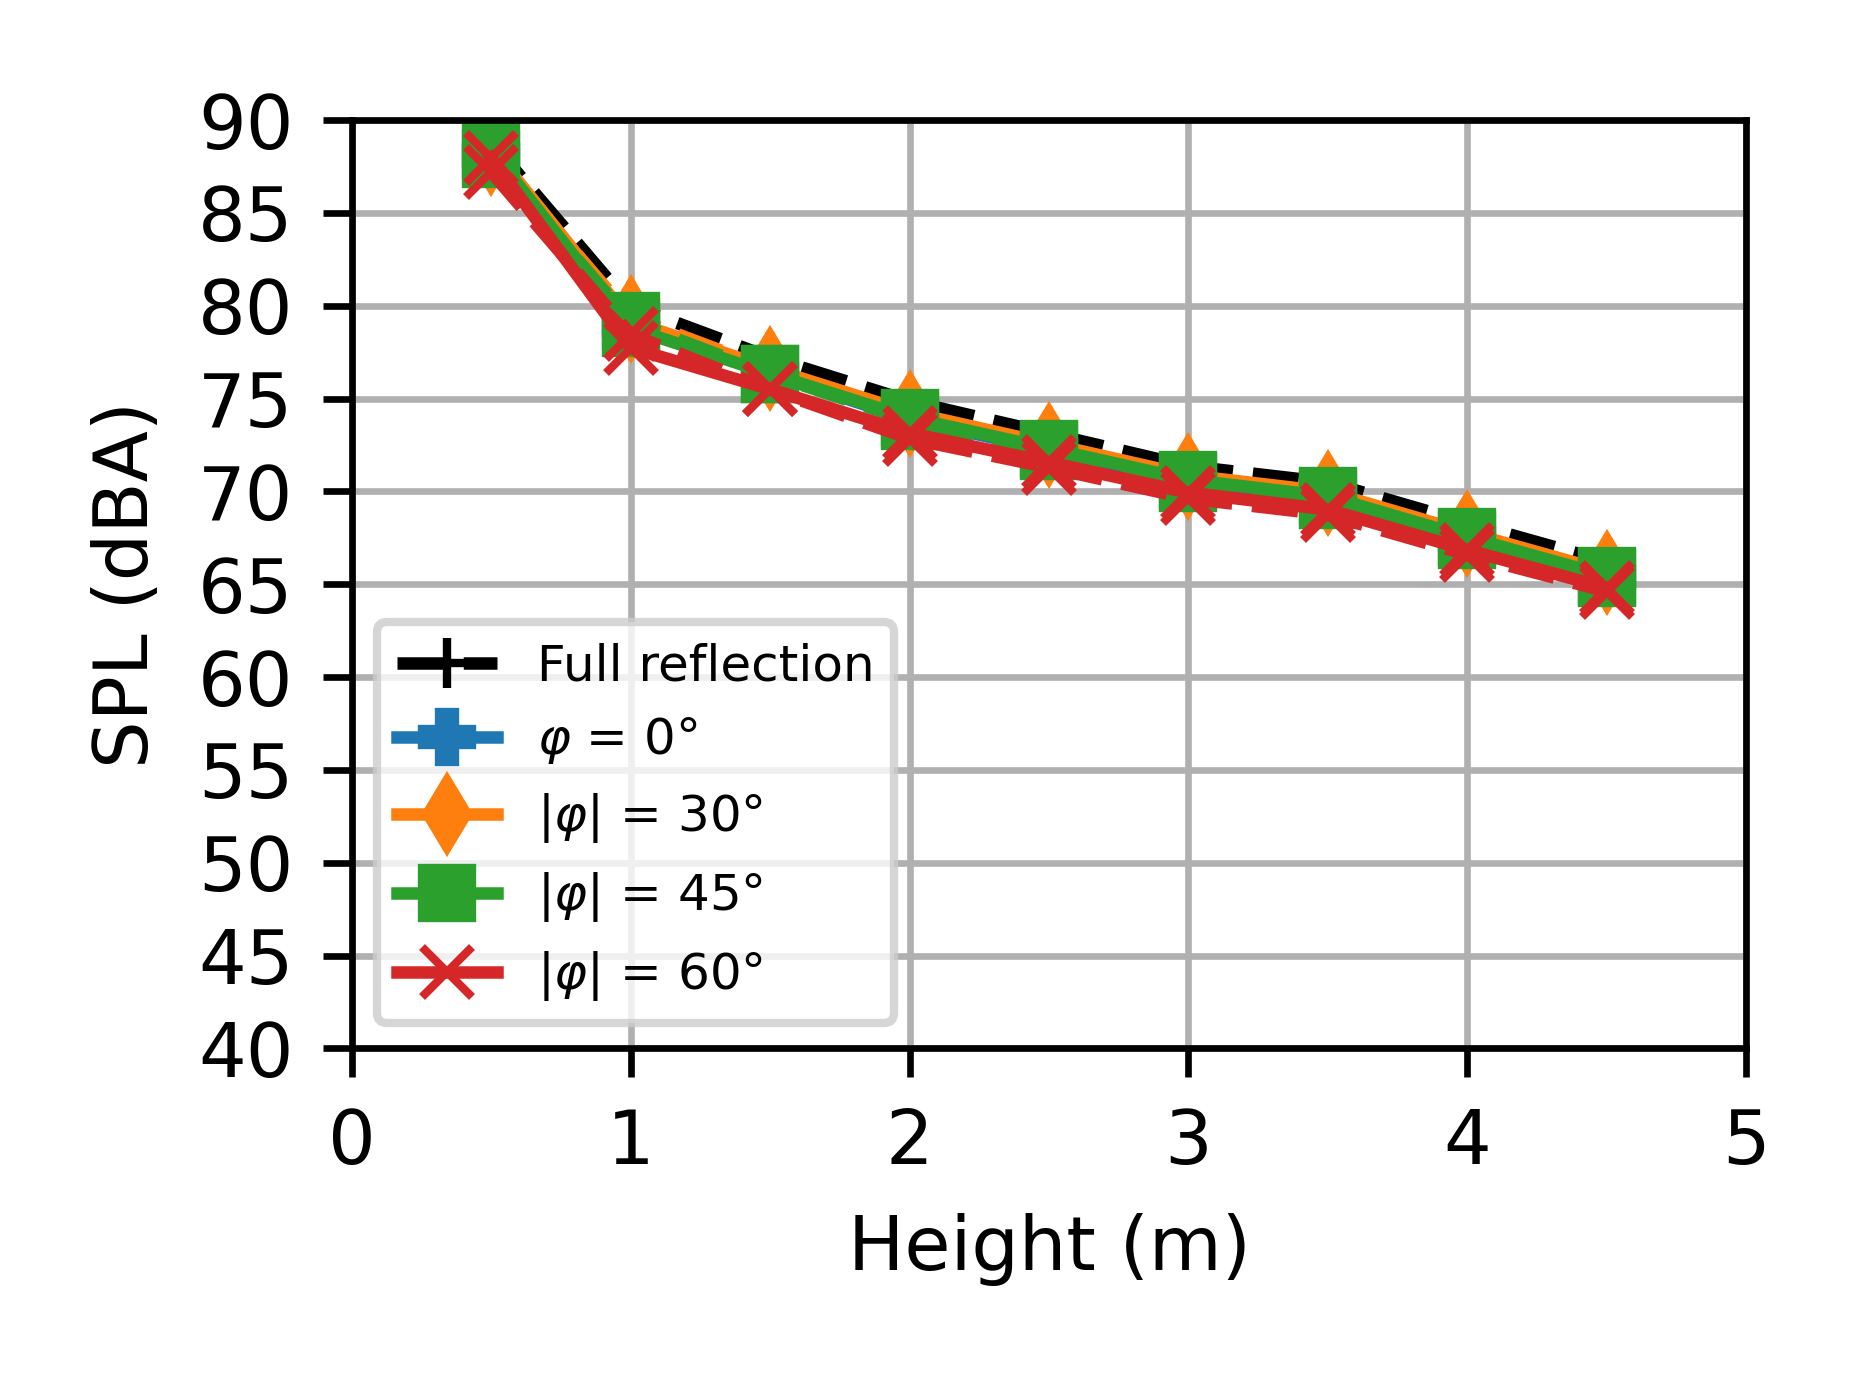
\includegraphics[width=0.49\textwidth]{fig/chap5/impedance/third_octave/SPL_2000_Hz.png}
		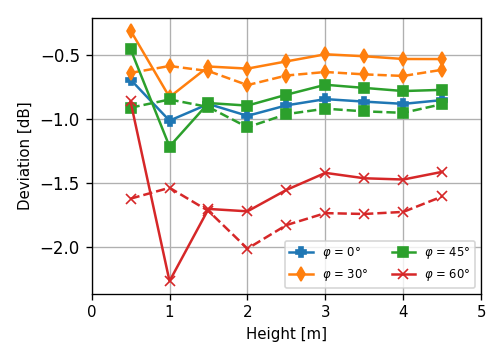
\includegraphics[width=0.49\textwidth]{fig/chap5/impedance/third_octave/deviation_2000_Hz.png}
		\caption{2000 Hz}
	\end{subfigure}

	\caption{Sound distribution at measurement position a, comparison between predictions obtained from the initial finite element model with the measurements. A-weighted SPL in one-third octave bands, dBA ref 20 $\mu$Pa.}
	\label{fig:third_octave_over_height_impedance}
\end{figure}

\begin{figure}[H]
	\centering
	\begin{subfigure}[b]{\textwidth}
		\centering
		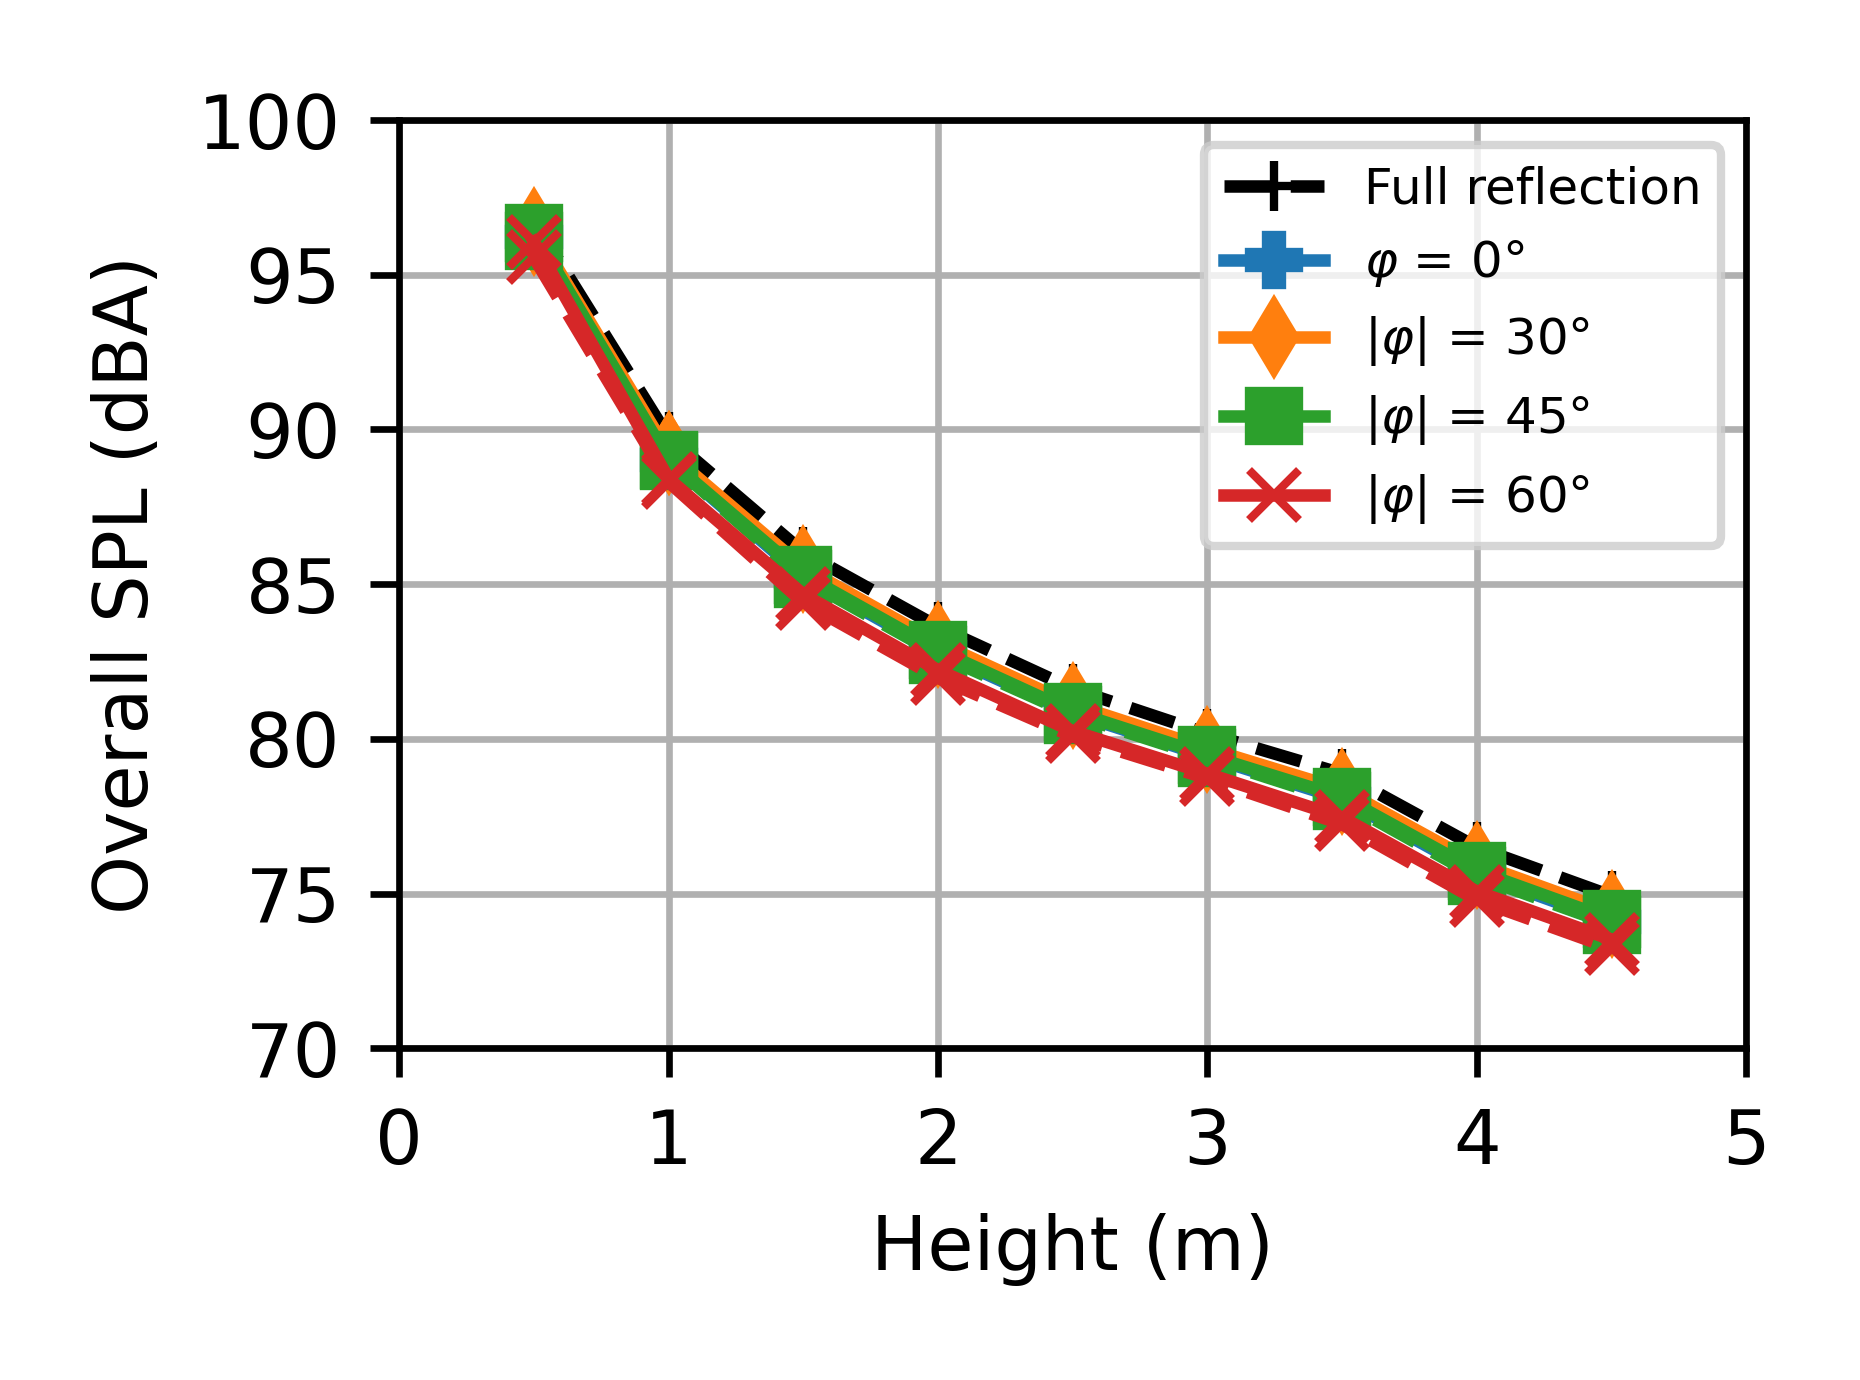
\includegraphics[width=0.49\textwidth]{fig/chap5/impedance/overall_SPL/overall_SPL_pos_a.png}
		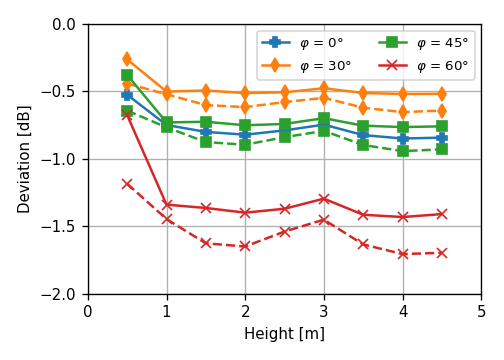
\includegraphics[width=0.49\textwidth]{fig/chap5/impedance/overall_SPL/deviation_pos_a.png}
		\caption{10 cm away from carbody}
	\end{subfigure}
	\begin{subfigure}[b]{\textwidth}
		\centering
		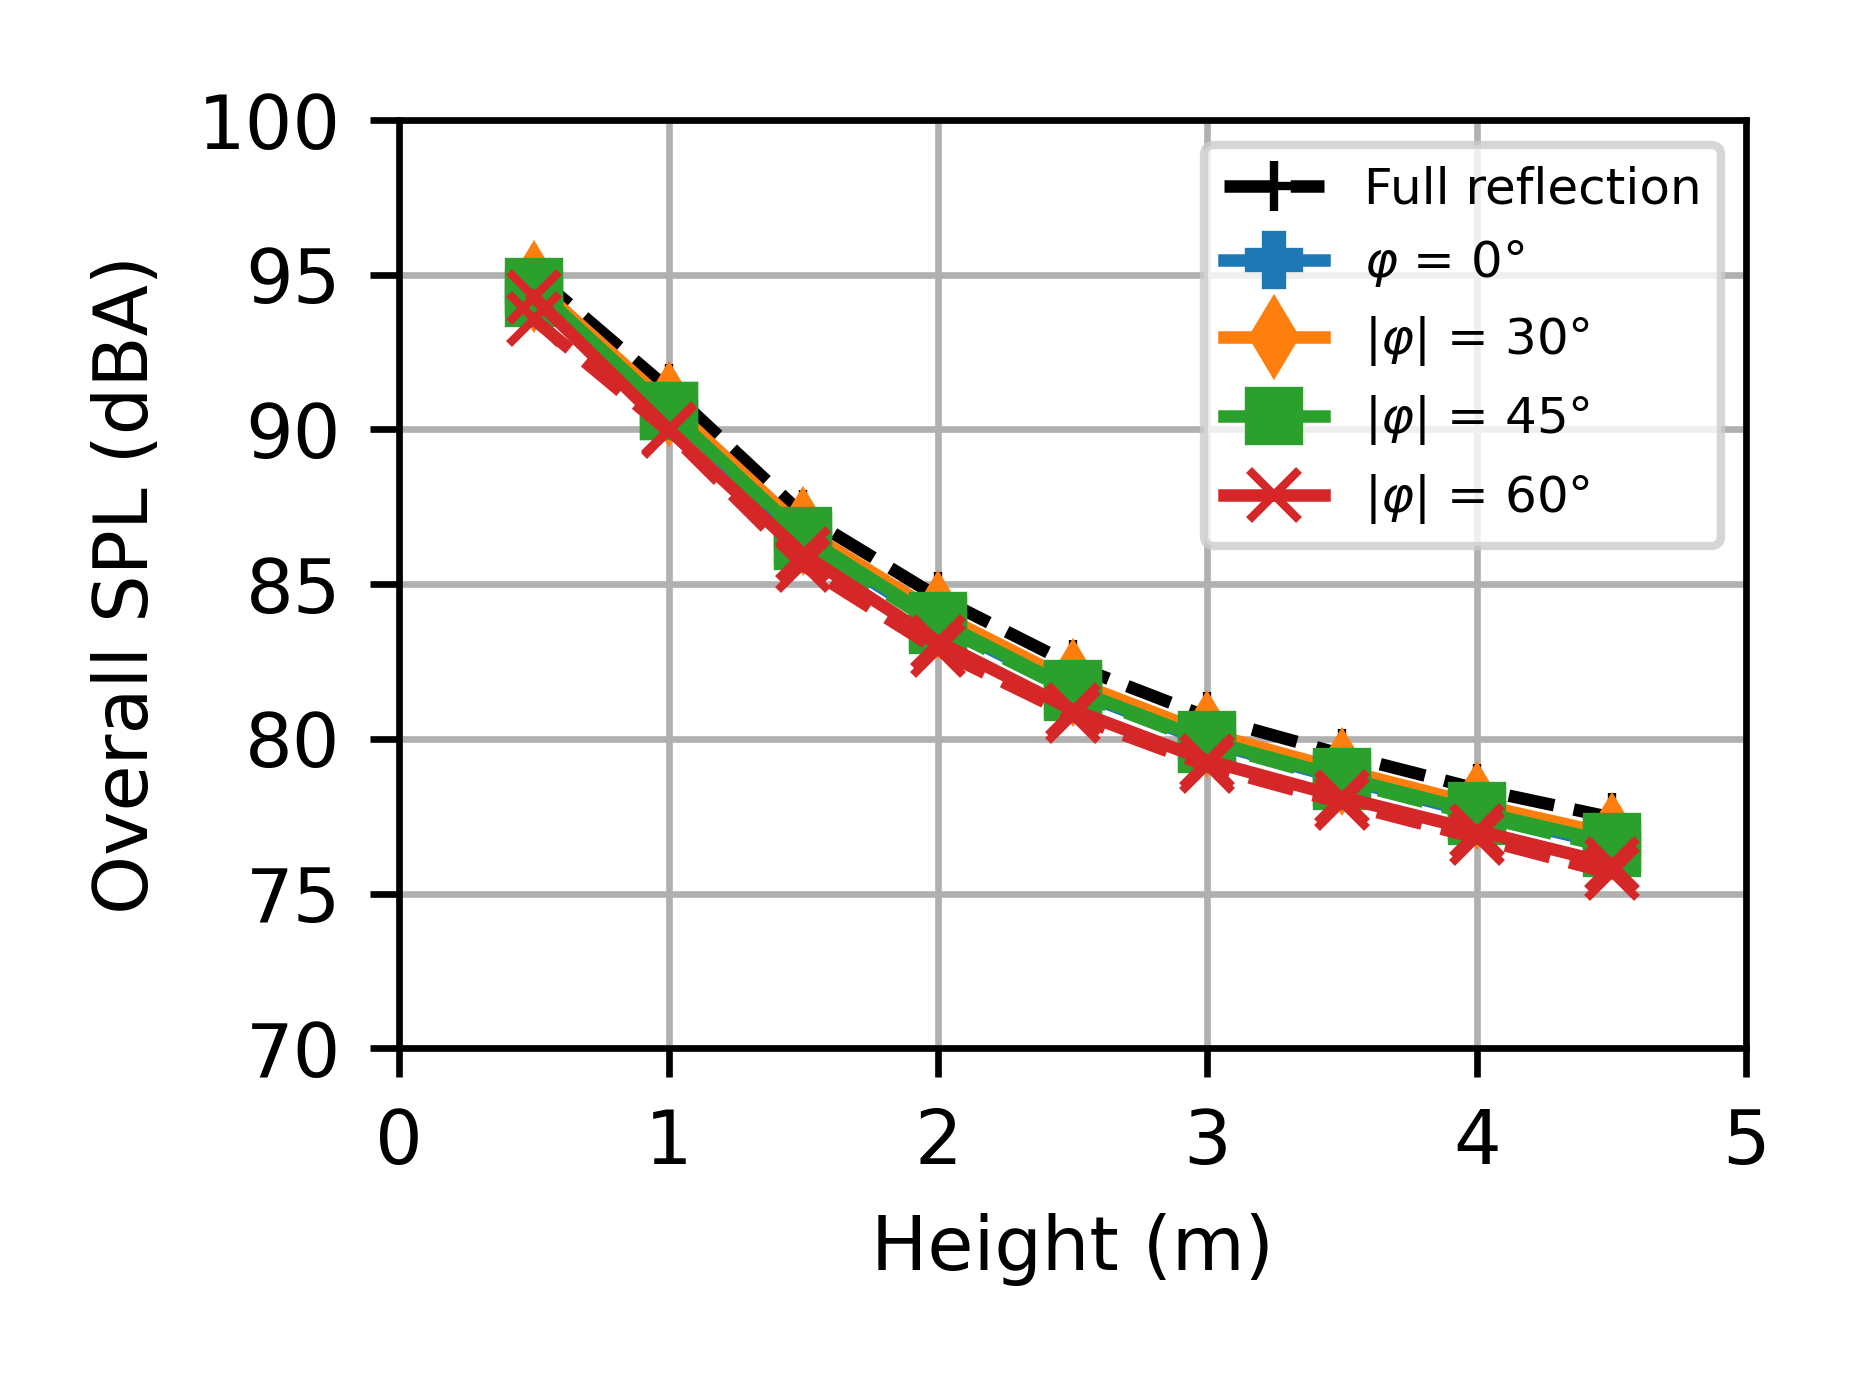
\includegraphics[width=0.49\textwidth]{fig/chap5/impedance/overall_SPL/overall_SPL_pos_f.png}
		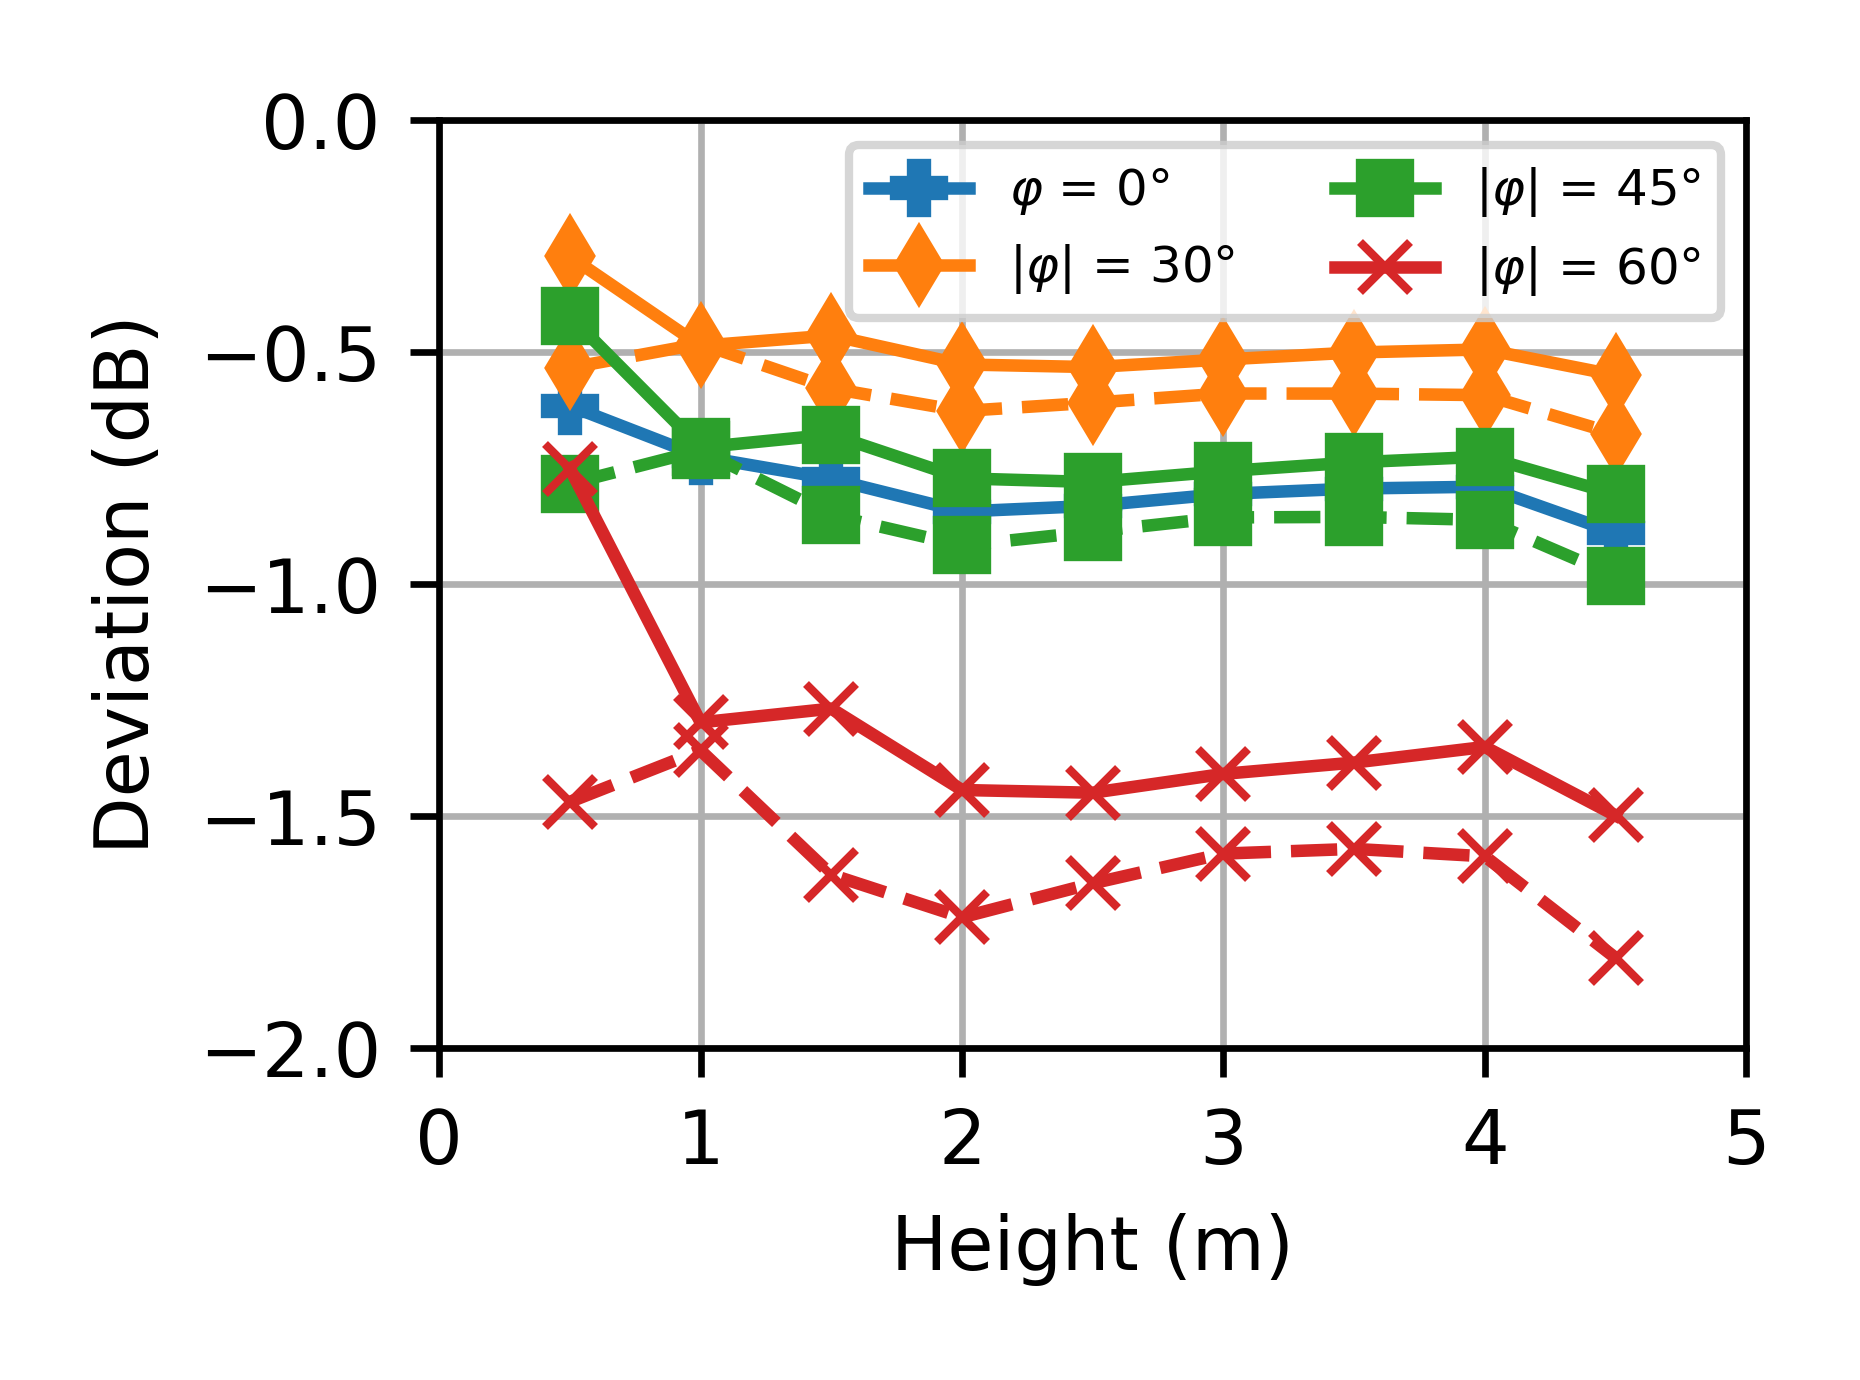
\includegraphics[width=0.49\textwidth]{fig/chap5/impedance/overall_SPL/deviation_pos_f.png}
		\caption{50 cm away from carbody}
	\end{subfigure}
	\begin{subfigure}[b]{\textwidth}
		\centering
		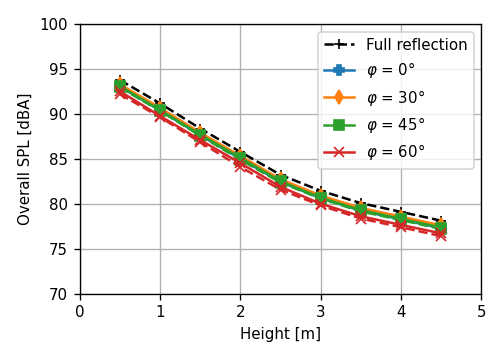
\includegraphics[width=0.49\textwidth]{fig/chap5/impedance/overall_SPL/overall_SPL_pos_g.png}
		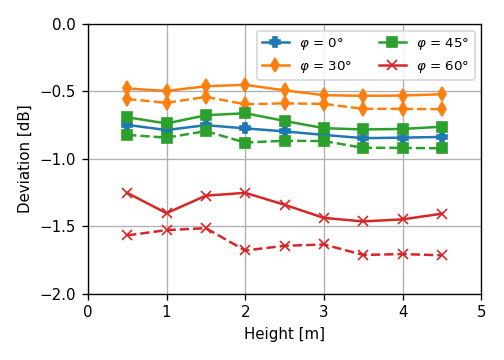
\includegraphics[width=0.49\textwidth]{fig/chap5/impedance/overall_SPL/deviation_pos_g.png}
		\caption{100 cm away from carbody}
	\end{subfigure}
	
	\caption{Sound distribution at measurement position a, comparison between predictions obtained from the initial finite element model with the measurements. A-weighted SPL in one-third octave bands, dBA ref 20 $\mu$Pa.}
	\label{fig:overall_SPL_impedance}
\end{figure}

\begin{figure}[H]
	\centering
	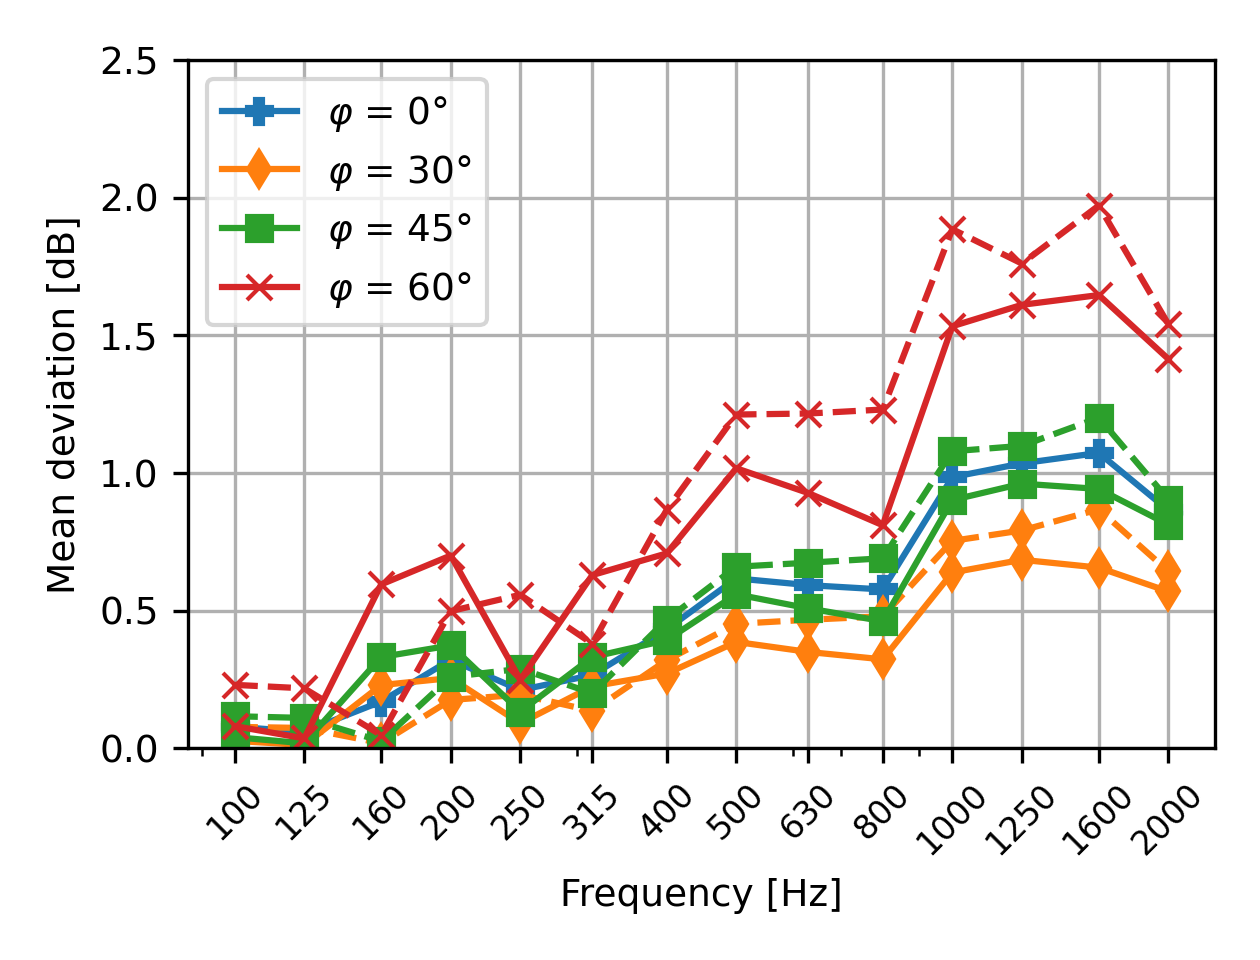
\includegraphics[width=0.7\linewidth]{fig/chap5/impedance/freq_spectrum/average_gap.png}
	\caption{Mean relative error compared to full reflective model in 1/3-octave band}
	\label{fig:gap_freq_spectrum_impedance}
\end{figure}


\section{Effect of varing frequency steps per 1/3-octave band}

\begin{figure}[H]
	\centering
	\begin{subfigure}[b]{0.49\textwidth}
		\centering
		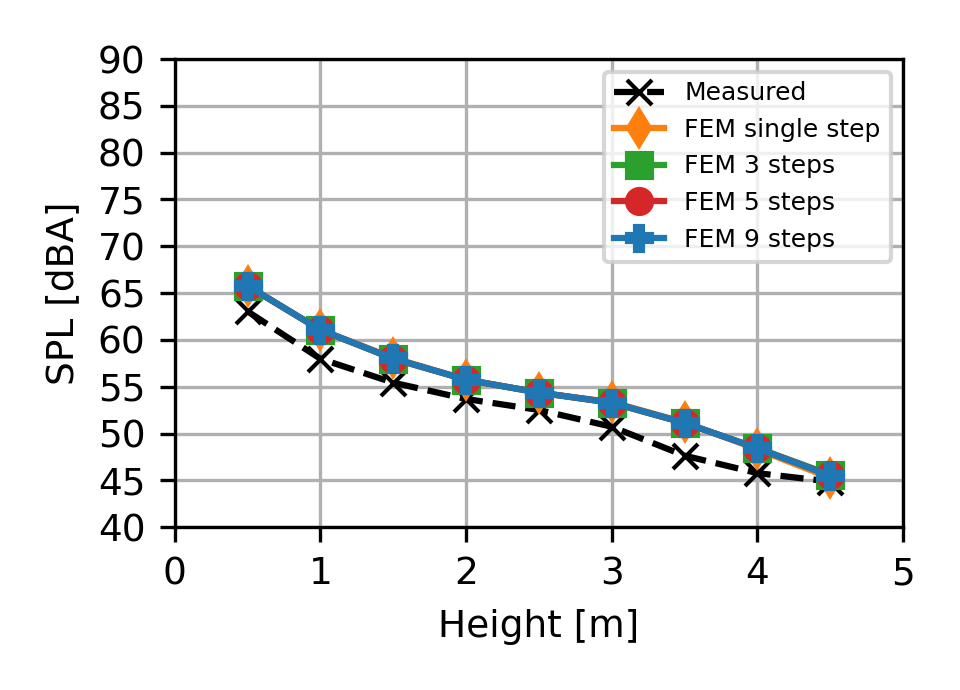
\includegraphics{fig/chap5/freq_steps/third_octave_over_height/100_Hz.png}
		\caption{100 Hz}
	\end{subfigure}
	\begin{subfigure}[b]{0.49\textwidth}
		\centering
		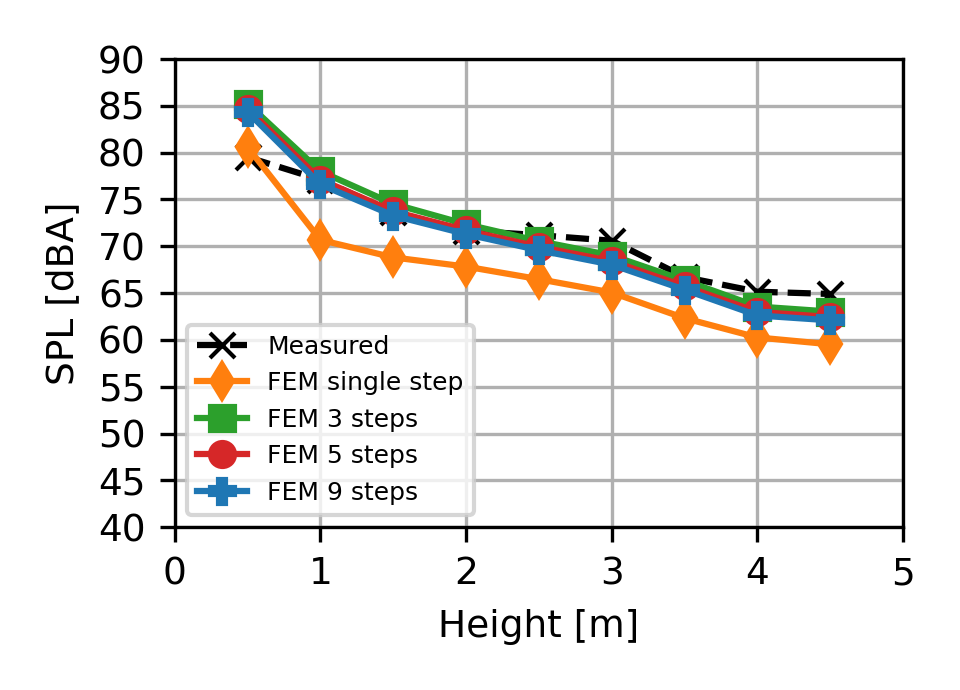
\includegraphics{fig/chap5/freq_steps/third_octave_over_height/315_Hz.png}
		\caption{315 Hz}
	\end{subfigure}
	\begin{subfigure}[b]{0.49\textwidth}
		\centering
		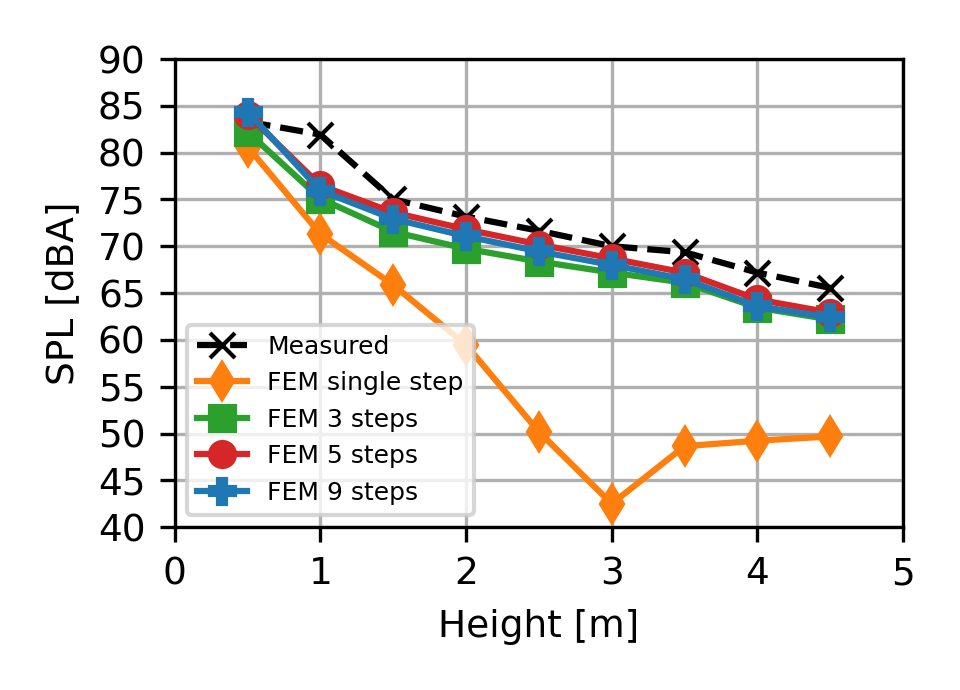
\includegraphics{fig/chap5/freq_steps/third_octave_over_height/630_Hz.png}
		\caption{630 Hz}
	\end{subfigure}
	\begin{subfigure}[b]{0.49\textwidth}
		\centering
		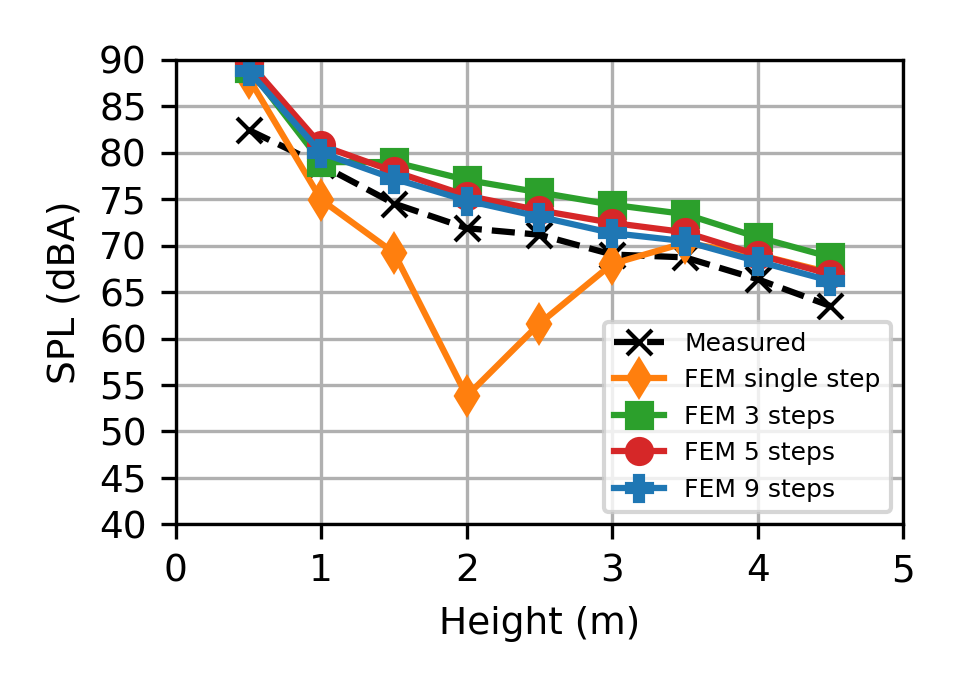
\includegraphics{fig/chap5/freq_steps/third_octave_over_height/2000_Hz.png}
		\caption{2000 Hz}
	\end{subfigure}
	
	\caption{Sound distribution at measurement position a, comparison between predictions obtained from the initial finite element model with the measurements. A-weighted SPL in one-third octave bands, dBA ref 20 $\mu$Pa.}
	\label{fig:third_octave_over_height_freq_steps}
\end{figure}


\begin{figure}[H]
	\centering
	\begin{subfigure}[b]{0.3\textwidth}
		\centering
		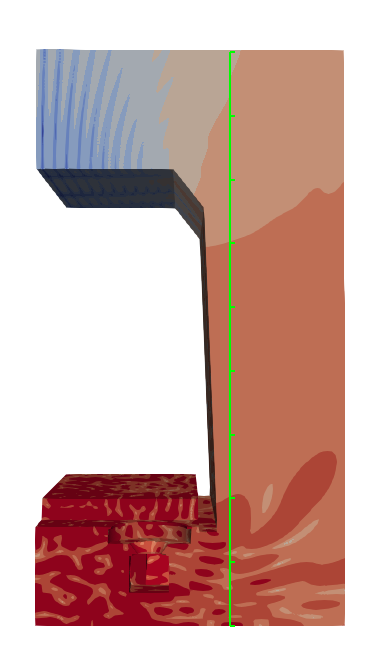
\includegraphics[width=\linewidth]{fig/chap5/freq_steps/field_result_1781Hz.png}
		\caption{1781 Hz}
	\end{subfigure}
	\hfill
	\begin{subfigure}[b]{0.3\textwidth}
		\centering
		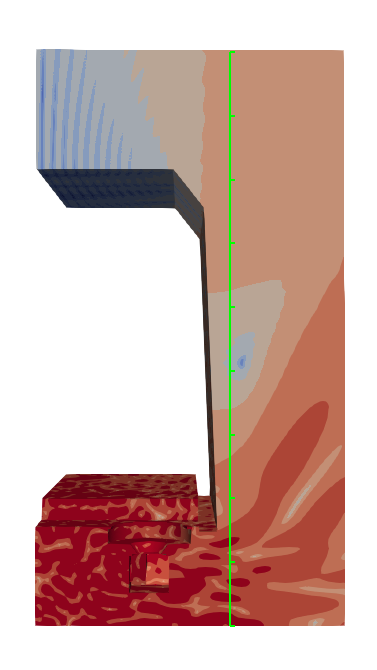
\includegraphics[width=\linewidth]{fig/chap5/freq_steps/field_result_2000Hz.png}
		\caption{2000 Hz}
	\end{subfigure}
	\hfill
	\begin{subfigure}[b]{0.3\textwidth}
		\centering
		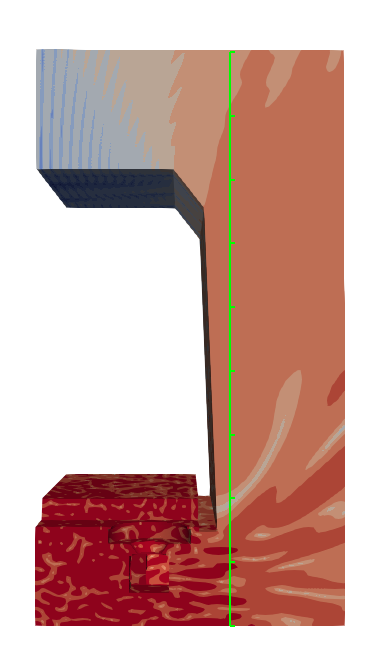
\includegraphics[width=\linewidth]{fig/chap5/freq_steps/field_result_2245Hz.png}
		\caption{2245 Hz}
	\end{subfigure}
	\caption{Pressure field of single frequency}
\end{figure}
